%!TEX root = paper.tex

\section{Metabolic Network Completion}\label{sec:problem}

Metabolism is the sum of all chemical reactions occurring within an organism.
As the products of a reaction may be reused as reactants, reactions can be chained to complex chemical pathways.
Such complex pathways are described by a metabolic network.

We represent a \emph{metabolic network} as a labeled directed bipartite graph
\(
G=(R\cup M,E,\StoichiometricFunction),
\)
where $R$ and $M$ are sets of nodes standing for \emph{reactions} and \emph{compounds} (also called metabolites), respectively.
%
When $(m,r)\in E$ or $(r,m)\in E$ for $m\in M$ and $r\in R$, the metabolite $m$ is called a \emph{reactant} or \emph{product} of reaction~$r$, respectively. \review{Metabolites and reactions nodes can both have multiple ingoing and outgoing edges.}
%
More formally, for any $r\in R$, define
\(
\Reactants{r}=\{m\in M\mid (m,r)\in E\}
\)
and
\(
\Products{r} =\{m\in M\mid (r,m)\in E\}
\).
%
%
The \emph{edge labeling}
\(
\StoichiometricFunction: E\rightarrow \mathbb{R}
\)
gives the stoichiometric coefficients of a reaction's reactants and products, respectively, i.e., their relative quantities involved in the reaction.
%
Finally, the activity rate of reactions is bound by lower and upper bounds,
denoted by $\MinFlux{r}\in\mathbb{R}^+_0$ and $\MaxFlux{r}\in\mathbb{R}^+_0$ for $r\in R$, respectively.
%
Whenever clear from the context,
we refer to metabolic networks with $G$ (or $G'$, etc) and denote the associated reactions and compounds with
$M$ and $R$ (or $M',R'$ etc), respectively.

We distinguish a set $S \subseteq M$ of compounds as initiation \emph{seeds}, that is,
compounds initially present due to experimental evidence.
%
Another set of compounds is assumed to be activated by default.
These \emph{boundary compounds} are defined as:
\(
\strseed(G) = \{ m\in M \mid r\in R,  m\in \Products{r}, \Reactants{r}=\emptyset \}
\).
%
For simplicity, we assume that all boundary compounds are seeds: $\strseed(G)\subseteq S$.
Note that follow-up concepts like reachability and activity in network completion are independent of this assumption.

For illustration, consider the metabolic network in Fig.~\ref{gra:toy_d}.
%
% ----------------------------------------------------------------------
\begin{figure}[t]
  \centering
    %!TEX root = paper.tex
\usetikzlibrary{shapes.misc, positioning}
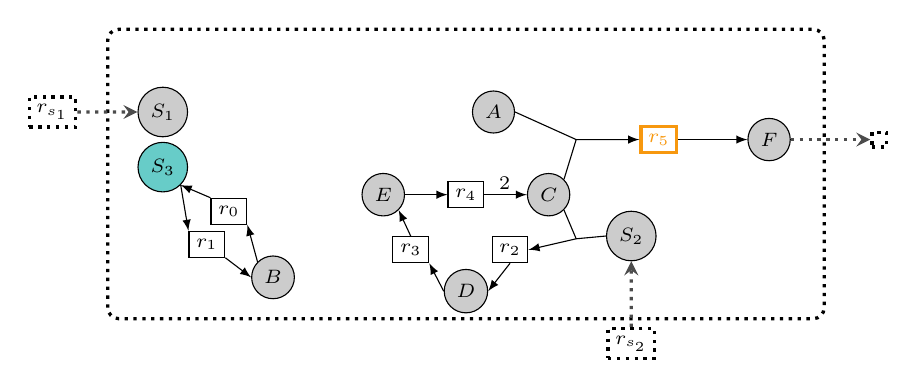
\begin{tikzpicture}[scale=0.7]\scriptsize
  \tikzstyle{metabolite}=[draw,circle,fill=white!80!black];
  \tikzstyle{repairmetabolite}=[draw,white!40!black, circle,fill=white!90!black,text=white!40!black,dashed];
  \tikzstyle{seed}=[draw,circle,fill=BlueGreen!70];%white!80!black
  \tikzstyle{target}=[draw,circle,fill=YellowOrange];%white!40!black
  \tikzstyle{reaction}=[draw,rectangle];
   \tikzstyle{export}=[draw,rectangle,dotted, very thick];
   \tikzstyle{exportrepair}=[draw,rectangle,dotted, very thick,white!80!black,text=white!70!black];
  \tikzstyle{repairreaction}=[draw,rectangle,white!40!black,text=white!40!black,dashed];
  \tikzstyle{initial}=[->,>=latex,thick];
  \tikzstyle{bdd}=[->,>=latex,thick];
  \tikzstyle{etiq}=[midway,fill=black!20,scale=0.5];
  \tikzstyle{stc}=[draw, rectangle, white, text=black]

  \node[stc] (stcr4C) at (6.2,6.7) {$2$};

  \draw [black,dotted, rounded corners, very thick] (-1,4.25) rectangle (12,9.5);
 % \node (system) [draw, rounded rectangle] at (0,0) {} (7cm,5cm);

  \node[seed] (S2) at (0,7) {$S_{3}$};
  \node[metabolite] (Sb2) at (8.5,5.75) {$S_{2}$};
  \node[metabolite] (S1) at (0,8) {$S_{1}$};

  \node[metabolite] (F) at (11,7.50) {$F$};

  \node[metabolite] (A) at (6,8) {$A$};
  \node[metabolite] (B) at (2,5.0) {$B$};
  \node[metabolite] (C) at (7,6.5) {$C$};
  \node[metabolite] (D) at (5.50,4.75) {$D$};
  \node[metabolite] (E) at (4,6.5) {$E$};
 % \node[repairmetabolite] (X) at (5,9) {$G$};

  \node[reaction] (R0) at (1.2,6.2) {$r_{0}$};
  \node[reaction] (R1) at (0.8,5.60) {$r_{1}$};
  \node[reaction] (R2) at (6.3,5.5) {$r_{2}$};
  \node[reaction] (R3) at (4.5,5.5) {$r_{3}$};
  \node[reaction] (R4) at (5.5,6.5) {$r_{4}$};
  \node[reaction, very thick,YellowOrange] (R5) at (9,7.50) {$r_{5}$}; %LimeGreen
  %\node[repairreaction] (R6) at (3,8) {$r_{6}$};
  %\node[repairreaction] (R7) at (2.3,6.9) {$r_{7}$};
  %\node[repairreaction] (R8) at (3,5.8) {$r_{8}$};
  %\node[repairreaction] (R9) at (8.5,8.5) {$r_{9}$};

  % R0 : S => B
  \draw[->,>=latex] (B.north west) -- (R0.south east);
  \draw[->,>=latex] (R0.north west) -- (S2.south east);

  % R1 : S <= B
  \draw[->,>=latex] (S2.south east) -- (R1.north west);
  \draw[->,>=latex] (R1.south east) -- (B.west);

  % R2 : Sb2+C => D
  \draw[->,>=latex] (Sb2.west) -- (7.5,5.70) -- (R2.east);
  \draw[] (C.south east) -- (7.5,5.70);
  \draw[->,>=latex] (R2.south) -- (D.east);

  % R3 : D => E
  \draw[->,>=latex] (D.west) -- (R3.south east);
  \draw[->,>=latex] (R3.north) -- (E.south east);

  % R4 : E => C
  \draw[->,>=latex] (E.east) -- (R4.west);
  \draw[->,>=latex] (R4.east) -- (C.west);

  % R5 : A+C => T
  \draw[->,>=latex] (A.east) -- (7.5,7.50) -- (R5.west);
  \draw[] (C.north east) -- (7.5,7.50);
  \draw[->,>=latex] (R5.east) -- (F.west);

  % R6 : S => A+X
 % \draw[->,>=latex,white!55!black,dashed] (S1.east) -- (R6.west);
  %\draw[->,>=latex,white!55!black,dashed] (R6.east) -- (4,8) -- (A.west);
  %\draw[->,>=latex,white!55!black,dashed] (4,8) -- (X.west);

  % R7 : S => E
 % \draw[->,>=latex,white!55!black,dashed] (S2.east) -- (R7.west);
  %\draw[->,>=latex,white!55!black,dashed] (R7.east) -- (E.north west);

  % R8 : B => E
 % \draw[->,>=latex,white!55!black,dashed] (B.north east) -- (R8.south west);
  %\draw[->,>=latex,white!55!black,dashed] (R8.east) -- (E.south);

  % R9 : X => F
 % \draw[->,>=latex,white!55!black,dashed] (X.east) -- (R9.north west);
  %\draw[->,>=latex,white!55!black,dashed] (R9.east) -- (F.north west);

  %export X
  %\node[exportrepair] (outX) at (6.5,10.30) {$r_{expX}$};
  %\draw[->,>=stealth,white!80!black,dotted, very thick] (X.north east) --  (outX.west);

  %export F
  \node[export] (outF) at (13,7.5) {\ExportReaction};
   \draw[->,>=stealth,white!30!black,dotted, very thick] (F.east) --  (outF.west);

  %import S2
   \node[export] (inS) at (-2,8) {$r_{s_1}$};
   \draw[->,>=stealth,white!30!black,dotted, very thick] (inS) --  (S1.west);

   %import Sb2
    \node[export] (inS2) at (8.5,3.8) {$r_{s_2}$};
    \draw[->,>=stealth,white!30!black,dotted, very thick] (inS2) --  (Sb2.south);

\end{tikzpicture}
%
%%% Local Variables:
%%% mode: latex
%%% TeX-master: "paper"
%%% End:

    \caption{Example of a metabolic network. Compounds and reactions are depicted by circles and rectangles respectively. Dashed reactions are reactions involving the boundary between the organism's metabolism and its environment. $r_5$ is the target reaction. $S_1$ and $S_2$ are boundary (and initiation) seeds. $S_3$ is assumed to be an initiation seed. Numbers on arrows describe the stoichiometry of reaction (default value is 1).}
    \label{gra:toy_d}
\end{figure}
% ----------------------------------------------------------------------
%
The network consists of 9 reactions, \SeedReaction, \SeedReactiont, \ExportReaction{} and $r_0$ to $r_5$, and 8 compounds, $A,\dots,F$, $S_1$, $S_2$ and $S_3$.
Here, $S=\{S_1,S_2,S_3\}$, $S_1$ and $S_2$ being the two boundary compounds of the network. Dashed rectangle describes the boundary of the system, outside of which is the environment of the organism.
%
Consider reaction
\(
r_4 : E\rightarrow 2C
\)
transforming one unit of $E$ into two units of $C$ (stoichiometric coefficients of 1 are omitted in the graphical representation; cf.~Fig.~\ref{gra:toy_d}).
%
We have
$\Reactants{r_4}=\{E\}$,
$\Products{r_4}=\{C\}$,
along with $\Stoichiometry{E}{r_4}=1 $
\ and $\Stoichiometry{r_4}{C}=2$.

In biology, several concepts have been introduced to model the activation of reaction fluxes in metabolic networks,
or to synthesize metabolic compounds.
%
To model this,
we introduce a function \ActivityFunction\ that given a metabolic network $G$ takes a set of seeds $S \subseteq M$ and returns a set of activated
reactions $\Activitytwo{G}{S} \subseteq R$.
%
%
% ----------------------------------------------------------------------
\begin{figure}[t]
  \centering
    %!TEX root = paper.tex
\usetikzlibrary{shapes.misc, positioning}
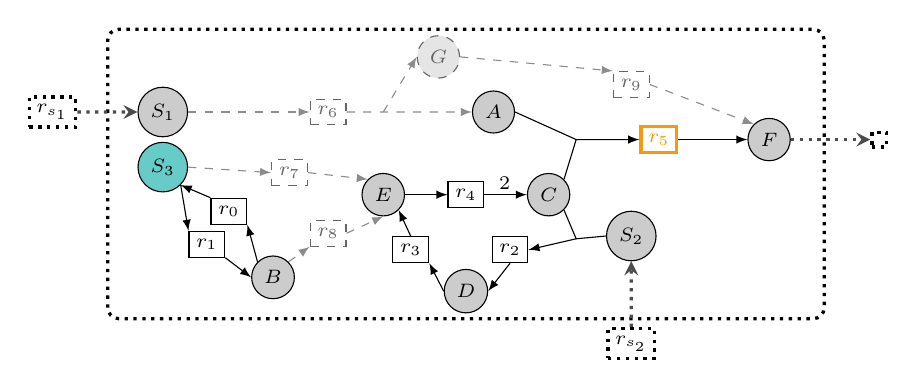
\begin{tikzpicture}[scale=0.7]\scriptsize
  \tikzstyle{metabolite}=[draw,circle,fill=white!80!black];
  \tikzstyle{repairmetabolite}=[draw,white!40!black, circle,fill=white!90!black,text=white!40!black,dashed];
  \tikzstyle{seed}=[draw,circle,fill=BlueGreen!70];%white!80!black
  \tikzstyle{target}=[draw,circle,fill=YellowOrange];%white!40!black
  \tikzstyle{reaction}=[draw,rectangle];
   \tikzstyle{export}=[draw,rectangle,dotted, very thick];
   \tikzstyle{exportrepair}=[draw,rectangle,dotted, very thick,white!80!black,text=white!70!black];
  \tikzstyle{repairreaction}=[draw,rectangle,white!40!black,text=white!40!black,dashed];
  \tikzstyle{initial}=[->,>=latex,thick];
  \tikzstyle{bdd}=[->,>=latex,thick];
  \tikzstyle{etiq}=[midway,fill=black!20,scale=0.5];
  \tikzstyle{stc}=[draw, rectangle, white, text=black]

  \node[stc] (stcr4C) at (6.2,6.7) {$2$};

  \draw [black,dotted, rounded corners, very thick] (-1,4.25) rectangle (12,9.5);
 % \node (system) [draw, rounded rectangle] at (0,0) {} (7cm,5cm);

  \node[seed] (S2) at (0,7) {$S_{3}$};
  \node[metabolite] (Sb2) at (8.5,5.75) {$S_{2}$};
  \node[metabolite] (S1) at (0,8) {$S_{1}$};

  \node[metabolite] (F) at (11,7.50) {$F$};

  \node[metabolite] (A) at (6,8) {$A$};
  \node[metabolite] (B) at (2,5.0) {$B$};
  \node[metabolite] (C) at (7,6.5) {$C$};
  \node[metabolite] (D) at (5.50,4.75) {$D$};
  \node[metabolite] (E) at (4,6.5) {$E$};
  \node[repairmetabolite] (X) at (5,9) {$G$};

  \node[reaction] (R0) at (1.2,6.2) {$r_{0}$};
  \node[reaction] (R1) at (0.8,5.60) {$r_{1}$};
  \node[reaction] (R2) at (6.3,5.5) {$r_{2}$};
  \node[reaction] (R3) at (4.5,5.5) {$r_{3}$};
  \node[reaction] (R4) at (5.5,6.5) {$r_{4}$};
  \node[reaction, very thick,YellowOrange] (R5) at (9,7.50) {$r_{5}$}; %LimeGreen
  \node[repairreaction] (R6) at (3,8) {$r_{6}$};
  \node[repairreaction] (R7) at (2.3,6.9) {$r_{7}$};
  \node[repairreaction] (R8) at (3,5.8) {$r_{8}$};
  \node[repairreaction] (R9) at (8.5,8.5) {$r_{9}$};

  % R0 : S => B
  \draw[->,>=latex] (B.north west) -- (R0.south east);
  \draw[->,>=latex] (R0.north west) -- (S2.south east);

  % R1 : S <= B
  \draw[->,>=latex] (S2.south east) -- (R1.north west);
  \draw[->,>=latex] (R1.south east) -- (B.west);

  % R2 : Sb2+C => D
  \draw[->,>=latex] (Sb2.west) -- (7.5,5.70) -- (R2.east);
  \draw[] (C.south east) -- (7.5,5.70);
  \draw[->,>=latex] (R2.south) -- (D.east);

  % R3 : D => E
  \draw[->,>=latex] (D.west) -- (R3.south east);
  \draw[->,>=latex] (R3.north) -- (E.south east);

  % R4 : E => C
  \draw[->,>=latex] (E.east) -- (R4.west);
  \draw[->,>=latex] (R4.east) -- (C.west);

  % R5 : A+C => T
  \draw[->,>=latex] (A.east) -- (7.5,7.50) -- (R5.west);
  \draw[] (C.north east) -- (7.5,7.50);
  \draw[->,>=latex] (R5.east) -- (F.west);

  % R6 : S => A+X
  \draw[->,>=latex,white!55!black,dashed] (S1.east) -- (R6.west);
  \draw[->,>=latex,white!55!black,dashed] (R6.east) -- (4,8) -- (A.west);
  \draw[->,>=latex,white!55!black,dashed] (4,8) -- (X.west);

  % R7 : S => E
  \draw[->,>=latex,white!55!black,dashed] (S2.east) -- (R7.west);
  \draw[->,>=latex,white!55!black,dashed] (R7.east) -- (E.north west);

  % R8 : B => E
  \draw[->,>=latex,white!55!black,dashed] (B.north east) -- (R8.south west);
  \draw[->,>=latex,white!55!black,dashed] (R8.east) -- (E.south);

  % R9 : X => F
  \draw[->,>=latex,white!55!black,dashed] (X.east) -- (R9.north west);
  \draw[->,>=latex,white!55!black,dashed] (R9.east) -- (F.north west);

  %export X
  %\node[exportrepair] (outX) at (6.5,10.30) {$r_{expX}$};
  %\draw[->,>=stealth,white!80!black,dotted, very thick] (X.north east) --  (outX.west);

  %export F
  \node[export] (outF) at (13,7.5) {\ExportReaction};
   \draw[->,>=stealth,white!30!black,dotted, very thick] (F.east) --  (outF.west);

   %import S2
    \node[export] (inS) at (-2,8) {$r_{s_1}$};
    \draw[->,>=stealth,white!30!black,dotted, very thick] (inS) --  (S1.west);

   %import Sb2
  \node[export] (inS2) at (8.5,3.8) {$r_{s_2}$};
  \draw[->,>=stealth,white!30!black,dotted, very thick] (inS2) --  (Sb2.south);

\end{tikzpicture}
%
%%% Local Variables:
%%% mode: latex
%%% TeX-master: "paper"
%%% End:

    \caption{Metabolic network completion problem. The purpose of its solving is to select the minimal number of reactions from a database (dashed shaded reactions) such that activation of target reaction $r_5$ is restored from boundary and/or initiation seeds. There are three formalisms for activation of target reaction: stoichiometric, topological and hybrid.}
    \label{gra:toy}
\end{figure}
% ----------------------------------------------------------------------
%
With it,
\emph{metabolic network completion} is about ensuring that a set of target reactions (reaction $r_5$ in~Fig.~\ref{gra:toy_d}) is activated from seed compounds in $S$
by possibly extending the metabolic network with reactions from a reference network (cf.\ shaded part in~Fig.~\ref{gra:toy}).

Formally, given
a metabolic network $G=(R\cup M,E,\StoichiometricFunction)$, % with bounds,
a set $S\subseteq M$ of seed compounds such that $\strseed(G) \subseteq S$,
a set $R_{T}\subseteq R$ of target reactions, and
a reference network $(R'\cup M',E',\StoichiometricFunction')$,
%
the \emph{metabolic network completion problem} is to find a set $R''\subseteq R'\setminus R$ of reactions of minimal size such that
\(
R_{T}\subseteq\Activitytwo{G''}{S}
\)
where%
\footnote{Since \StoichiometricFunction, $\StoichiometricFunction'$ have disjoint domains we view them as relations and compose them by union.}
\begin{align}
  \label{eq:completion:graph}
  G''&= ((R\cup R'')\cup (M\cup M''),E\cup E'',\StoichiometricFunction'')\ ,
  \\\label{eq:completion:metabolites}
  M''&=\{m\in M'\mid r\in R'', m\in\Reactants{r}\cup\Products{r}\}\ ,
  \\\label{eq:completion:edges}
  E''&=E'\cap((M''\times R'')\cup(R''\times M'')) , \text{ and}
  \\
  \StoichiometricFunction''&=\StoichiometricFunction\cup\StoichiometricFunction'
  \ .
\end{align}
%
We call $R''$ a \emph{completion} of $(R\cup M,E,\StoichiometricFunction)$ from $(R'\cup M',E',\StoichiometricFunction')$ wrt $S$ and $R_{T}$.
%
Our concept of activation allows different biological paradigms to be captured.
%
Accordingly,
different formulations of metabolic network completion can be characterized:
the stoichiometric, the relaxed stoichiometric, the topological, and the hybrid one.
We elaborate upon their formal characterizations in the following sections.

\subsection{Stoichiometric Metabolic Network Completion}\label{sec:stoichio} %\emph
%
The first activation semantics has been introduced in the context of Flux Balance Analysis
capturing reaction flux distributions of metabolic networks at steady state.
%
In this paradigm, each reaction $r$ is associated with a \emph{metabolic flux value},
expressed as a real variable $v_r$ confined by the minimum and maximum rates:
%
\begin{align} \label{eq:stoichiometric:bounds}
  & \MinFlux{r} \leq  v_r\leq \MaxFlux{r} \qquad\text{ for } r\in R.
\end{align}
%
Flux distributions are formalized in terms of a system of equations relying on the stoichiometric coefficients of reactions.
%
\review{Reaction stoichiometries are governed by the \emph{law of mass conservation} under a steady state assumption; in other words, the mass of the system remains constant over the reaction.
The input and output fluxes of reactions consuming and producing a metabolite are balanced.}
%
\begin{align}
\label{eq:stoichiometric:equation}
  & \textstyle
    \sum_{\substack{r\in R}}\Stoichiometry{r}{m}\cdot v_r
    +
    \sum_{\substack{r\in R}}-\Stoichiometry{m}{r}\cdot v_r
    =
    0
    \qquad \text{ for } m\in M.
\end{align}
%
Given a target reaction $r_T\in R_T$, a metabolic network $G=(R\cup M,E,\StoichiometricFunction)$ and a set of seeds $S$,
\emph{stoichiometric activation} is defined as follows:
\begin{align}%*
\label{eq:stoichiometric:activation}
  r_T \in \Activity{s}{G}{S} & \ \text{ iff } \ v_{r_T} >0 \text{ and }
                               \eqref{eq:stoichiometric:bounds} \text{ and } \eqref{eq:stoichiometric:equation}\text{ hold for }M\text{ and }R.
\end{align}%*
Note that the condition $v_{r_T} >0$ strengthens the flux condition for $r_T\in R$ in the second part.
More generally, observe that activated target reactions are not directly related to the network's seeds $S$.
However,
the activation of targets highly depends on the boundary compounds in $\strseed(G)$
for which \eqref{eq:stoichiometric:equation} \review{is always satisfied and thus initiates the fluxes.
Since boundary compounds are produced by at least one reaction without prerequisite,
an arbitrary amount might be produced.
Therefore, the incoming flux value always balances the sum of the flux values associated to outgoing edges.
Intuitively, boundary compounds are nutrients that are expected to be available in the system
for the consumption by the metabolic network,
thus initiating the reactions within.}
%
In our draft network $G$,
consisting of all \review{non-dashed} nodes and edges depicted in Fig.~\ref{gra:toy}
(viz.\ reactions \SeedReaction, \SeedReactiont, \ExportReaction{} and $r_0$ to $r_5$ and compounds $A,\dots,F$, $S_1$, $S_2$, and $S_3$ and $r_5$ the single target reaction)
and the reference network $G'$,
consisting of the shaded part of Fig~\ref{gra:toy},
(viz.\ reactions $r_6$ to $r_9$ and metabolite $G$)
a strict stoichiometry-based completion aims to obtain a solution with $r_5\in\Activity{s}{G''}{\{S_1,S_2,S_3\}}$ where $v_{r_5}$ is maximal.
%
This can be achieved by adding the completion $R''_1=\{r_{6},r_9\}$ (Fig.~\ref{gra:toy_ss}).
%
\review{The cycle made of compounds $E,C,D$ and the boundary seed $S_2$ is already balanced and notably self-activated.
Indeed, initiation of $D$ and $E$ producibility requires the producibility of $C$ (in addition to the presence of the boundary seed $S_2$) that itself depends on $D$ and $E$. Yet, according the flux conditions, that models steady state conditions, the cycle is activated.
Such self-activation of cyclic pathways is an inherent problem of purely stoichiometric approaches to network completion.
This is a drawback of the semantics because the effective activation of the cycle requires the additional (and unchecked) condition that at least one of the compounds was present as the initial state of the system. This could be the case provided there exist another way to enable the production of one or several components of the cycle (here an activable reaction producing $E$ for instance) \citep{Prigent2017}.}
%
The instance of Equation~\eqref{eq:stoichiometric:equation} controlling the reaction rates related to metabolite $C$ is
\(
2\cdot v_{r_4} - v_{r_2} - v_{r_5} = 0
\).


To solve metabolic network completion with flux-balance activated reactions,
Linear Programming can be used to maximize the flux rate $v_{r_T}$ provided that the linear constraints are satisfied.
%
Nonetheless, this problem turns out to be hard to solve in practice and existing approaches scale poorly to real-life applications (cf.~ \citep{Orth2010}).

This motivated the use of approximate methods.
%
The relaxed problem is obtained by weakening the mass-balance equation \eqref{eq:stoichiometric:equation} as follows:
%
\begin{align}
\label{eq:stoichiometric:equation:relaxed}
  &  \textstyle        \sum_{\substack{r\in R}} \Stoichiometry{r}{m}\cdot v_r
                       +
                       \sum_{\substack{r\in R}}-\Stoichiometry{m}{r}\cdot v_r
                       \geq
                       0
                       \qquad \text{ for } m\in M.
\end{align}
%
This lets us define the concept of \emph{relaxed stoichiometric activation}:
\begin{align}%*
\label{eq:stoichiometric:activation:relaxed}
  r_T \in \Activity{r}{G}{S} & \ \text{ iff } \ v_{r_T} >0 \text{ and }
                               \eqref{eq:stoichiometric:bounds} \text{ and } \eqref{eq:stoichiometric:equation:relaxed}\text{ hold for }M\text{ and }R.
\end{align}%*
The resulting problem can now be efficiently solved with Linear Programming~\citep{SatishKumar2007}.
%
Existing systems addressing strict stoichiometric network completion either
cannot guarantee optimal solutions~\citep{laten2014a} or
do not support a focus on specific target reactions~\citep{Thiele2014}.
Other approaches either partially relax the problem~\citep{Vitkin2012} or
solve the relaxed problem based on Equation~\eqref{eq:stoichiometric:equation:relaxed},
like the popular system \gapfill~\citep{SatishKumar2007}. Applied to the network of Fig.~\ref{gra:toy}, the minimal completion under the relaxed stoichiometric activation is $R''_1=\{r_{6}\}$  (Fig.~\ref{gra:toy_sr}) but does not carry flux because of the accumulation of metabolite $G$, allowed by Equation~\eqref{eq:stoichiometric:equation:relaxed}.
%
Note however that for strict steady-state modeling an \textit{a posteriori} verification of solutions is needed
to warrant the exact mass-balance equation~\eqref{eq:stoichiometric:equation}.


% ----------------------------------------------------------------------
\begin{figure}
    \captionsetup{width=0.45\textwidth}
    \centering
    \begin{minipage}[t]{.5\textwidth}
      \centering
      %!TEX root = paper.tex
\usetikzlibrary{shapes.misc, positioning}
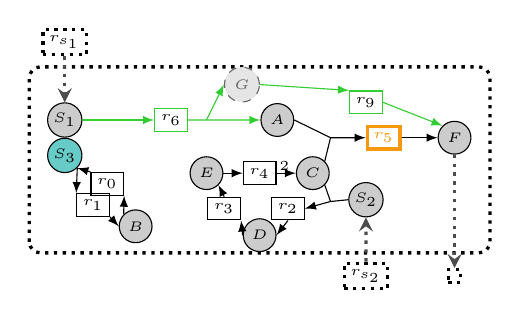
\begin{tikzpicture}[scale=0.45]\tiny
  \tikzstyle{metabolite}=[draw,circle,fill=white!80!black, text width=0.4cm, inner sep=0pt, align=center];
  \tikzstyle{repairmetabolite}=[draw,white!40!black, circle,fill=white!90!black,text=white!40!black,dashed];
  \tikzstyle{seed}=[draw,circle,fill=BlueGreen!70, text width=0.4cm, inner sep=0pt, align=center];%white!80!black
  \tikzstyle{target}=[draw,circle,fill=YellowOrange];%white!40!black
  \tikzstyle{reaction}=[draw,rectangle];
   \tikzstyle{export}=[draw,rectangle,dotted, very thick];
   \tikzstyle{exportrepair}=[draw,rectangle,dotted, very thick,white!80!black,text=white!70!black];
  \tikzstyle{repairreaction}=[draw,rectangle,white!40!black,text=white!40!black,dashed];
  \tikzstyle{solreaction}=[draw,rectangle,LimeGreen,text=black];
  \tikzstyle{initial}=[->,>=latex,thick];
  \tikzstyle{bdd}=[->,>=latex,thick];
  \tikzstyle{etiq}=[midway,fill=black!20,scale=0.5];
  \tikzstyle{stc}=[draw, rectangle, white, text=black]

  \node[stc] (stcr4C) at (6.2,6.7) {$2$};

  \draw [black,dotted, rounded corners, very thick] (-1,4.25) rectangle (12,9.5);
 % \node (system) [draw, rounded rectangle] at (0,0) {} (7cm,5cm);

  \node[seed] (S2) at (0,7) {$S_{3}$};
  \node[metabolite] (Sb2) at (8.5,5.75) {$S_{2}$};
  \node[metabolite] (S1) at (0,8) {$S_{1}$};

  \node[metabolite] (F) at (11,7.50) {$F$};

  \node[metabolite] (A) at (6,8) {$A$};
  \node[metabolite] (B) at (2,5.0) {$B$};
  \node[metabolite] (C) at (7,6.5) {$C$};
  \node[metabolite] (D) at (5.50,4.75) {$D$};
  \node[metabolite] (E) at (4,6.5) {$E$};
  \node[repairmetabolite] (X) at (5,9) {$G$};

  \node[reaction] (R0) at (1.2,6.2) {$r_{0}$};
  \node[reaction] (R1) at (0.8,5.60) {$r_{1}$};
  \node[reaction] (R2) at (6.3,5.5) {$r_{2}$};
  \node[reaction] (R3) at (4.5,5.5) {$r_{3}$};
  \node[reaction] (R4) at (5.5,6.5) {$r_{4}$};
  \node[reaction, very thick,YellowOrange] (R5) at (9,7.50) {$r_{5}$}; %LimeGreen
  \node[solreaction] (R6) at (3,8) {$r_{6}$};
  % \node[repairreaction] (R7) at (2.3,6.9) {$r_{7}$};
  % \node[repairreaction] (R8) at (3,5.8) {$r_{8}$};
  \node[solreaction] (R9) at (8.5,8.5) {$r_{9}$};

  % R0 : S => B
  \draw[->,>=latex] (B.north west) -- (R0.south east);
  \draw[->,>=latex] (R0.north west) -- (S2.south east);

  % R1 : S <= B
  \draw[->,>=latex] (S2.south east) -- (R1.north west);
  \draw[->,>=latex] (R1.south east) -- (B.west);

  % R2 : Sb2+C => D
  \draw[->,>=latex] (Sb2.west) -- (7.5,5.70) -- (R2.east);
  \draw[] (C.south east) -- (7.5,5.70);
  \draw[->,>=latex] (R2.south) -- (D.east);

  % R3 : D => E
  \draw[->,>=latex] (D.west) -- (R3.south east);
  \draw[->,>=latex] (R3.north) -- (E.south east);

  % R4 : E => C
  \draw[->,>=latex] (E.east) -- (R4.west);
  \draw[->,>=latex] (R4.east) -- (C.west);

  % R5 : A+C => T
  \draw[->,>=latex] (A.east) -- (7.5,7.50) -- (R5.west);
  \draw[] (C.north east) -- (7.5,7.50);
  \draw[->,>=latex] (R5.east) -- (F.west);

  % R6 : S => A+X
  \draw[->,>=latex,LimeGreen] (S1.east) -- (R6.west);
  \draw[->,>=latex,LimeGreen] (R6.east) -- (4,8) -- (A.west);
  \draw[->,>=latex,LimeGreen] (4,8) -- (X.west);

  % % R7 : S => E
  % \draw[->,>=latex,white!55!black,dashed] (S2.east) -- (R7.west);
  % \draw[->,>=latex,white!55!black,dashed] (R7.east) -- (E.north west);
  %
  % % R8 : B => E
  % \draw[->,>=latex,white!55!black,dashed] (B.north east) -- (R8.south west);
  % \draw[->,>=latex,white!55!black,dashed] (R8.east) -- (E.south);

  % R9 : X => F
  \draw[->,>=latex,LimeGreen] (X.east) -- (R9.north west);
  \draw[->,>=latex,LimeGreen] (R9.east) -- (F.north west);

  %export X
  %\node[exportrepair] (outX) at (6.5,10.30) {$r_{expX}$};
  %\draw[->,>=stealth,white!80!black,dotted, very thick] (X.north east) --  (outX.west);

  %export F
  \node[export] (outF) at (11,3.6) {\ExportReaction};
   \draw[->,>=stealth,white!30!black,dotted, very thick] (F.south) --  (outF.north);

  %import S2
   \node[export] (inS) at (0,10.2) {$r_{s_1}$};
   \draw[->,>=stealth,white!30!black,dotted, very thick] (inS.south) --  (S1.north);

   %import Sb2
  \node[export] (inS2) at (8.5,3.6) {$r_{s_2}$};
  \draw[->,>=stealth,white!30!black,dotted, very thick] (inS2) --  (Sb2.south);

\end{tikzpicture}
%
%%% Local Variables:
%%% mode: latex
%%% TeX-master: "paper"
%%% End:

      \caption{Solution to metabolic network completion under stoichiometric activation hypothesis in order to satisfy Equations~\eqref{eq:stoichiometric:bounds},~\eqref{eq:stoichiometric:equation} and ~\eqref{eq:stoichiometric:activation}. Within this network, there exists at least one flux distribution which activates $r_5$.}
      \label{gra:toy_ss}
    \end{minipage}%
    \begin{minipage}[t]{.5\textwidth}
      \centering
      %!TEX root = paper.tex
\usetikzlibrary{shapes.misc, positioning}
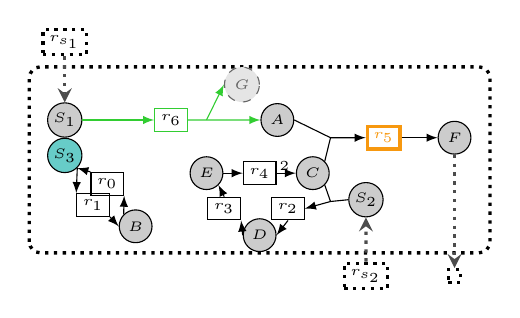
\begin{tikzpicture}[scale=0.45]\tiny
  \tikzstyle{metabolite}=[draw,circle,fill=white!80!black, text width=0.4cm, inner sep=0pt, align=center];
  \tikzstyle{repairmetabolite}=[draw,white!40!black, circle,fill=white!90!black,text=white!40!black,dashed];
  \tikzstyle{seed}=[draw,circle,fill=BlueGreen!70, text width=0.4cm, inner sep=0pt, align=center];%white!80!black
  \tikzstyle{target}=[draw,circle,fill=YellowOrange];%white!40!black
  \tikzstyle{reaction}=[draw,rectangle];
   \tikzstyle{export}=[draw,rectangle,dotted, very thick];
   \tikzstyle{exportrepair}=[draw,rectangle,dotted, very thick,white!80!black,text=white!70!black];
  \tikzstyle{repairreaction}=[draw,rectangle,white!40!black,text=white!40!black,dashed];
  \tikzstyle{solreaction}=[draw,rectangle,LimeGreen,text=black];
  \tikzstyle{initial}=[->,>=latex,thick];
  \tikzstyle{bdd}=[->,>=latex,thick];
  \tikzstyle{etiq}=[midway,fill=black!20,scale=0.5];
  \tikzstyle{stc}=[draw, rectangle, white, text=black]

  \node[stc] (stcr4C) at (6.2,6.7) {$2$};

  \draw [black,dotted, rounded corners, very thick] (-1,4.25) rectangle (12,9.5);
 % \node (system) [draw, rounded rectangle] at (0,0) {} (7cm,5cm);

  \node[seed] (S2) at (0,7) {$S_{3}$};
  \node[metabolite] (Sb2) at (8.5,5.75) {$S_{2}$};
  \node[metabolite] (S1) at (0,8) {$S_{1}$};

  \node[metabolite] (F) at (11,7.50) {$F$};

  \node[metabolite] (A) at (6,8) {$A$};
  \node[metabolite] (B) at (2,5.0) {$B$};
  \node[metabolite] (C) at (7,6.5) {$C$};
  \node[metabolite] (D) at (5.50,4.75) {$D$};
  \node[metabolite] (E) at (4,6.5) {$E$};
  \node[repairmetabolite] (X) at (5,9) {$G$};

  \node[reaction] (R0) at (1.2,6.2) {$r_{0}$};
  \node[reaction] (R1) at (0.8,5.60) {$r_{1}$};
  \node[reaction] (R2) at (6.3,5.5) {$r_{2}$};
  \node[reaction] (R3) at (4.5,5.5) {$r_{3}$};
  \node[reaction] (R4) at (5.5,6.5) {$r_{4}$};
  \node[reaction, very thick,YellowOrange] (R5) at (9,7.50) {$r_{5}$}; %LimeGreen
  \node[solreaction] (R6) at (3,8) {$r_{6}$};
  % \node[repairreaction] (R7) at (2.3,6.9) {$r_{7}$};
  % \node[repairreaction] (R8) at (3,5.8) {$r_{8}$};
  % \node[repairreaction] (R9) at (8.5,8.5) {$r_{9}$};

  % R0 : S => B
  \draw[->,>=latex] (B.north west) -- (R0.south east);
  \draw[->,>=latex] (R0.north west) -- (S2.south east);

  % R1 : S <= B
  \draw[->,>=latex] (S2.south east) -- (R1.north west);
  \draw[->,>=latex] (R1.south east) -- (B.west);

  % R2 : Sb2+C => D
  \draw[->,>=latex] (Sb2.west) -- (7.5,5.70) -- (R2.east);
  \draw[] (C.south east) -- (7.5,5.70);
  \draw[->,>=latex] (R2.south) -- (D.east);

  % R3 : D => E
  \draw[->,>=latex] (D.west) -- (R3.south east);
  \draw[->,>=latex] (R3.north) -- (E.south east);

  % R4 : E => C
  \draw[->,>=latex] (E.east) -- (R4.west);
  \draw[->,>=latex] (R4.east) -- (C.west);

  % R5 : A+C => T
  \draw[->,>=latex] (A.east) -- (7.5,7.50) -- (R5.west);
  \draw[] (C.north east) -- (7.5,7.50);
  \draw[->,>=latex] (R5.east) -- (F.west);

  % R6 : S => A+X
  \draw[->,>=latex,LimeGreen] (S1.east) -- (R6.west);
  \draw[->,>=latex,LimeGreen] (R6.east) -- (4,8) -- (A.west);
  \draw[->,>=latex,LimeGreen] (4,8) -- (X.west);

  % % R7 : S => E
  % \draw[->,>=latex,white!55!black,dashed] (S2.east) -- (R7.west);
  % \draw[->,>=latex,white!55!black,dashed] (R7.east) -- (E.north west);
  %
  % % R8 : B => E
  % \draw[->,>=latex,white!55!black,dashed] (B.north east) -- (R8.south west);
  % \draw[->,>=latex,white!55!black,dashed] (R8.east) -- (E.south);

  % % R9 : X => F
  % \draw[->,>=latex,green] (X.east) -- (R9.north west);
  % \draw[->,>=latex,green] (R9.east) -- (F.north west);

  %export X
  %\node[exportrepair] (outX) at (6.5,10.30) {$r_{expX}$};
  %\draw[->,>=stealth,white!80!black,dotted, very thick] (X.north east) --  (outX.west);

  %export F
  \node[export] (outF) at (11,3.6) {\ExportReaction};
   \draw[->,>=stealth,white!30!black,dotted, very thick] (F.south) --  (outF.north);

  %import S2
   \node[export] (inS) at (0,10.2) {$r_{s_1}$};
   \draw[->,>=stealth,white!30!black,dotted, very thick] (inS.south) --  (S1.north);

   %import Sb2
  \node[export] (inS2) at (8.5,3.6) {$r_{s_2}$};
  \draw[->,>=stealth,white!30!black,dotted, very thick] (inS2) --  (Sb2.south);

\end{tikzpicture}
%
%%% Local Variables:
%%% mode: latex
%%% TeX-master: "paper"
%%% End:

      \caption{Solution to metabolic network completion under relaxed stoichiometric activation hypothesis in order to satisfy Equations~\eqref{eq:stoichiometric:bounds},~\eqref{eq:stoichiometric:equation:relaxed} and ~\eqref{eq:stoichiometric:activation:relaxed}. Notice that within this completed network, there exist no flux distribution allowing the reaction $r_5$ to be activated.}
      \label{gra:toy_sr}
    \end{minipage}
\end{figure}
% ----------------------------------------------------------------------

\subsection{Topological Metabolic Network Completion}\label{sec:topo} %emph
%
A qualitative approach to metabolic network completion relies on the topology of networks for capturing the activation of reactions.
%
Given a metabolic network $G$, a reaction $r\in R$ is \emph{activated} from a set of seeds $S$ if all reactants in $\Reactants{r}$ are reachable from~$S$.
%
Moreover, a metabolite $m\in M$ is \emph{reachable} from $S$ if %
$m\in S$
or if
$m\in\Products{r}$ for some reaction $r\in R$ where all $m'\in\Reactants{r}$ are reachable from~$S$.
%
The \emph{scope} of $S$, written $\Sigma_G(S)$, is the closure of compounds reachable from~$S$.
%
In this setting, \emph{topological activation} of reactions from a set of seeds $S$ is defined as follows:
%
\begin{align}%*
  r_T \in \Activity{t}{G}{S} \ \text{ iff } \ \Reactants{r_T} \subseteq \Sigma_G(S).   \label{eq:topological:activation}
\end{align} %*
%
Note that this semantics avoids self-activated cycles by imposing an external entry sufficient to initiate all cycles ($S_3$ is not enough to activate the cycle as it does not activate one of its reaction on its own).
The resulting network completion problem can be expressed as a combinatorial optimization problem and effectively solved with ASP~\citep{schthi09a}.

For illustration, consider again the draft and reference networks $G$ and $G'$ in Fig.~\ref{gra:toy_d} and Fig.~\ref{gra:toy}.
%
We get $\Sigma_{G}(\{S_1,S_2,S_3\})=\{S_1,S_2,S_3,B\}$, indicating that target reaction $r_5$ is not activated from the seeds with the draft network
because $A$ and $C$, its reactants, are not reachable.
%
This changes once the network is completed.
%
Valid minimal completions are $R''_2=\{r_6,r_7\}$ (Fig.~\ref{gra:toy_st1}) and $R''_3=\{r_6,r_8\}$ (Fig.~\ref{gra:toy_st2}) because
\(
r_5\in\Activity{t}{G''_i}{\{S_1,S_2\}}\mbox{ since }\{A,C\}\subseteq\Sigma_{G''_i}(\{S_1,S_2\})
\)
for all extended networks $G''_i$ obtained from completions $R''_i$ of $G$ for $i\in\{2,3\}$.
%
% ----------------------------------------------------------------------
\begin{figure}
    \captionsetup{width=0.45\textwidth}
    \centering
    \begin{minipage}[t]{.5\textwidth}
      \centering
      %!TEX root = paper.tex
\usetikzlibrary{shapes.misc, positioning}
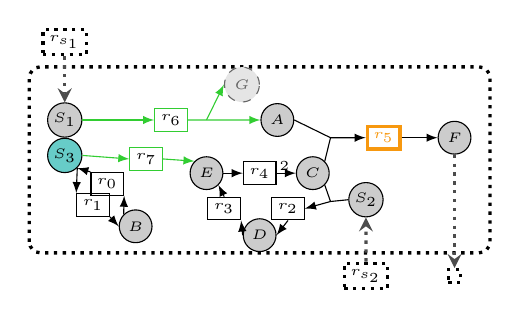
\begin{tikzpicture}[scale=0.45]\tiny
  \tikzstyle{metabolite}=[draw,circle,fill=white!80!black, text width=0.4cm, inner sep=0pt, align=center];
  \tikzstyle{repairmetabolite}=[draw,white!40!black, circle,fill=white!90!black,text=white!40!black,dashed];
  \tikzstyle{seed}=[draw,circle,fill=BlueGreen!70, text width=0.4cm, inner sep=0pt, align=center];%white!80!black
  \tikzstyle{target}=[draw,circle,fill=YellowOrange];%white!40!black
  \tikzstyle{reaction}=[draw,rectangle];
   \tikzstyle{export}=[draw,rectangle,dotted, very thick];
   \tikzstyle{exportrepair}=[draw,rectangle,dotted, very thick,white!80!black,text=white!70!black];
  \tikzstyle{repairreaction}=[draw,rectangle,white!40!black,text=white!40!black,dashed];
  \tikzstyle{solreaction}=[draw,rectangle,LimeGreen,text=black];
  \tikzstyle{initial}=[->,>=latex,thick];
  \tikzstyle{bdd}=[->,>=latex,thick];
  \tikzstyle{etiq}=[midway,fill=black!20,scale=0.5];
  \tikzstyle{stc}=[draw, rectangle, white, text=black]

  \node[stc] (stcr4C) at (6.2,6.7) {$2$};

  \draw [black,dotted, rounded corners, very thick] (-1,4.25) rectangle (12,9.5);
 % \node (system) [draw, rounded rectangle] at (0,0) {} (7cm,5cm);

  \node[seed] (S2) at (0,7) {$S_{3}$};
  \node[metabolite] (Sb2) at (8.5,5.75) {$S_{2}$};
  \node[metabolite] (S1) at (0,8) {$S_{1}$};

  \node[metabolite] (F) at (11,7.50) {$F$};

  \node[metabolite] (A) at (6,8) {$A$};
  \node[metabolite] (B) at (2,5.0) {$B$};
  \node[metabolite] (C) at (7,6.5) {$C$};
  \node[metabolite] (D) at (5.50,4.75) {$D$};
  \node[metabolite] (E) at (4,6.5) {$E$};
  \node[repairmetabolite] (X) at (5,9) {$G$};

  \node[reaction] (R0) at (1.2,6.2) {$r_{0}$};
  \node[reaction] (R1) at (0.8,5.60) {$r_{1}$};
  \node[reaction] (R2) at (6.3,5.5) {$r_{2}$};
  \node[reaction] (R3) at (4.5,5.5) {$r_{3}$};
  \node[reaction] (R4) at (5.5,6.5) {$r_{4}$};
  \node[reaction, very thick,YellowOrange] (R5) at (9,7.50) {$r_{5}$}; %LimeGreen
  \node[solreaction] (R6) at (3,8) {$r_{6}$};
  \node[solreaction] (R7) at (2.3,6.9) {$r_{7}$};
  % \node[repairreaction] (R8) at (3,5.8) {$r_{8}$};
  % \node[repairreaction] (R9) at (8.5,8.5) {$r_{9}$};

  % R0 : S => B
  \draw[->,>=latex] (B.north west) -- (R0.south east);
  \draw[->,>=latex] (R0.north west) -- (S2.south east);

  % R1 : S <= B
  \draw[->,>=latex] (S2.south east) -- (R1.north west);
  \draw[->,>=latex] (R1.south east) -- (B.west);

  % R2 : Sb2+C => D
  \draw[->,>=latex] (Sb2.west) -- (7.5,5.70) -- (R2.east);
  \draw[] (C.south east) -- (7.5,5.70);
  \draw[->,>=latex] (R2.south) -- (D.east);

  % R3 : D => E
  \draw[->,>=latex] (D.west) -- (R3.south east);
  \draw[->,>=latex] (R3.north) -- (E.south east);

  % R4 : E => C
  \draw[->,>=latex] (E.east) -- (R4.west);
  \draw[->,>=latex] (R4.east) -- (C.west);

  % R5 : A+C => T
  \draw[->,>=latex] (A.east) -- (7.5,7.50) -- (R5.west);
  \draw[] (C.north east) -- (7.5,7.50);
  \draw[->,>=latex] (R5.east) -- (F.west);

  % R6 : S => A+X
  \draw[->,>=latex,LimeGreen] (S1.east) -- (R6.west);
  \draw[->,>=latex,LimeGreen] (R6.east) -- (4,8) -- (A.west);
  \draw[->,>=latex,LimeGreen] (4,8) -- (X.west);

  % R7 : S => E
  \draw[->,>=latex,LimeGreen] (S2.east) -- (R7.west);
  \draw[->,>=latex,LimeGreen] (R7.east) -- (E.north west);
  %
  % % R8 : B => E
  % \draw[->,>=latex,white!55!black,dashed] (B.north east) -- (R8.south west);
  % \draw[->,>=latex,white!55!black,dashed] (R8.east) -- (E.south);

  % % R9 : X => F
  % \draw[->,>=latex,green] (X.east) -- (R9.north west);
  % \draw[->,>=latex,green] (R9.east) -- (F.north west);

  %export X
  %\node[exportrepair] (outX) at (6.5,10.30) {$r_{expX}$};
  %\draw[->,>=stealth,white!80!black,dotted, very thick] (X.north east) --  (outX.west);

  %export F
  \node[export] (outF) at (11,3.6) {\ExportReaction};
   \draw[->,>=stealth,white!30!black,dotted, very thick] (F.south) --  (outF.north);

  %import S2
   \node[export] (inS) at (0,10.2) {$r_{s_1}$};
   \draw[->,>=stealth,white!30!black,dotted, very thick] (inS.south) --  (S1.north);

   %import Sb2
  \node[export] (inS2) at (8.5,3.6) {$r_{s_2}$};
  \draw[->,>=stealth,white!30!black,dotted, very thick] (inS2) --  (Sb2.south);

\end{tikzpicture}
%
%%% Local Variables:
%%% mode: latex
%%% TeX-master: "paper"
%%% End:

      \caption{First solution to metabolic network completion under topological activation hypothesis satisfying Equation~\eqref{eq:topological:activation}. The production of C cannot be explained by a self-activated cycle and requires an external source of compounds via $S_3$ and reaction $r_7$.}
      \label{gra:toy_st1}
    \end{minipage}%
    \begin{minipage}[t]{.5\textwidth}
      \centering
      %!TEX root = paper.tex
\usetikzlibrary{shapes.misc, positioning}
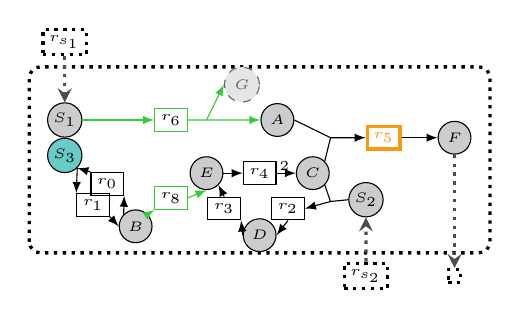
\begin{tikzpicture}[scale=0.45]\tiny
  \tikzstyle{metabolite}=[draw,circle,fill=white!80!black, text width=0.4cm, inner sep=0pt, align=center];
  \tikzstyle{repairmetabolite}=[draw,white!40!black, circle,fill=white!90!black,text=white!40!black,dashed];
  \tikzstyle{seed}=[draw,circle,fill=BlueGreen!70, text width=0.4cm, inner sep=0pt, align=center];%white!80!black
  \tikzstyle{target}=[draw,circle,fill=YellowOrange];%white!40!black
  \tikzstyle{reaction}=[draw,rectangle];
   \tikzstyle{export}=[draw,rectangle,dotted, very thick];
   \tikzstyle{exportrepair}=[draw,rectangle,dotted, very thick,white!80!black,text=white!70!black];
  \tikzstyle{repairreaction}=[draw,rectangle,white!40!black,text=white!40!black,dashed];
  \tikzstyle{solreaction}=[draw,rectangle,LimeGreen,text=black];
  \tikzstyle{initial}=[->,>=latex,thick];
  \tikzstyle{bdd}=[->,>=latex,thick];
  \tikzstyle{etiq}=[midway,fill=black!20,scale=0.5];
  \tikzstyle{stc}=[draw, rectangle, white, text=black]

  \node[stc] (stcr4C) at (6.2,6.7) {$2$};

  \draw [black,dotted, rounded corners, very thick] (-1,4.25) rectangle (12,9.5);
 % \node (system) [draw, rounded rectangle] at (0,0) {} (7cm,5cm);

  \node[seed] (S2) at (0,7) {$S_{3}$};
  \node[metabolite] (Sb2) at (8.5,5.75) {$S_{2}$};
  \node[metabolite] (S1) at (0,8) {$S_{1}$};

  \node[metabolite] (F) at (11,7.50) {$F$};

  \node[metabolite] (A) at (6,8) {$A$};
  \node[metabolite] (B) at (2,5.0) {$B$};
  \node[metabolite] (C) at (7,6.5) {$C$};
  \node[metabolite] (D) at (5.50,4.75) {$D$};
  \node[metabolite] (E) at (4,6.5) {$E$};
  \node[repairmetabolite] (X) at (5,9) {$G$};

  \node[reaction] (R0) at (1.2,6.2) {$r_{0}$};
  \node[reaction] (R1) at (0.8,5.60) {$r_{1}$};
  \node[reaction] (R2) at (6.3,5.5) {$r_{2}$};
  \node[reaction] (R3) at (4.5,5.5) {$r_{3}$};
  \node[reaction] (R4) at (5.5,6.5) {$r_{4}$};
  \node[reaction, very thick,YellowOrange] (R5) at (9,7.50) {$r_{5}$}; %LimeGreen
  \node[solreaction] (R6) at (3,8) {$r_{6}$};
  % \node[solreaction] (R7) at (2.3,6.9) {$r_{7}$};
  \node[solreaction] (R8) at (3,5.8) {$r_{8}$};
  % \node[repairreaction] (R9) at (8.5,8.5) {$r_{9}$};

  % R0 : S => B
  \draw[->,>=latex] (B.north west) -- (R0.south east);
  \draw[->,>=latex] (R0.north west) -- (S2.south east);

  % R1 : S <= B
  \draw[->,>=latex] (S2.south east) -- (R1.north west);
  \draw[->,>=latex] (R1.south east) -- (B.west);

  % R2 : Sb2+C => D
  \draw[->,>=latex] (Sb2.west) -- (7.5,5.70) -- (R2.east);
  \draw[] (C.south east) -- (7.5,5.70);
  \draw[->,>=latex] (R2.south) -- (D.east);

  % R3 : D => E
  \draw[->,>=latex] (D.west) -- (R3.south east);
  \draw[->,>=latex] (R3.north) -- (E.south east);

  % R4 : E => C
  \draw[->,>=latex] (E.east) -- (R4.west);
  \draw[->,>=latex] (R4.east) -- (C.west);

  % R5 : A+C => T
  \draw[->,>=latex] (A.east) -- (7.5,7.50) -- (R5.west);
  \draw[] (C.north east) -- (7.5,7.50);
  \draw[->,>=latex] (R5.east) -- (F.west);

  % R6 : S => A+X
  \draw[->,>=latex,LimeGreen] (S1.east) -- (R6.west);
  \draw[->,>=latex,LimeGreen] (R6.east) -- (4,8) -- (A.west);
  \draw[->,>=latex,LimeGreen] (4,8) -- (X.west);

  % % R7 : S => E
  % \draw[->,>=latex,white!55!black,dashed] (S2.east) -- (R7.west);
  % \draw[->,>=latex,white!55!black,dashed] (R7.east) -- (E.north west);

  % R8 : B => E
  \draw[->,>=latex,LimeGreen] (B.north east) -- (R8.south west);
  \draw[->,>=latex,LimeGreen] (R8.east) -- (E.south);

  % % R9 : X => F
  % \draw[->,>=latex,green] (X.east) -- (R9.north west);
  % \draw[->,>=latex,green] (R9.east) -- (F.north west);

  %export X
  %\node[exportrepair] (outX) at (6.5,10.30) {$r_{expX}$};
  %\draw[->,>=stealth,white!80!black,dotted, very thick] (X.north east) --  (outX.west);

  %export F
  \node[export] (outF) at (11,3.6) {\ExportReaction};
   \draw[->,>=stealth,white!30!black,dotted, very thick] (F.south) --  (outF.north);

  %import S2
   \node[export] (inS) at (0,10.2) {$r_{s_1}$};
   \draw[->,>=stealth,white!30!black,dotted, very thick] (inS.south) --  (S1.north);

   %import Sb2
  \node[export] (inS2) at (8.5,3.6) {$r_{s_2}$};
  \draw[->,>=stealth,white!30!black,dotted, very thick] (inS2) --  (Sb2.south);

\end{tikzpicture}
%
%%% Local Variables:
%%% mode: latex
%%% TeX-master: "paper"
%%% End:

      \caption{Second solution to metabolic network completion under topological activation hypothesis satisfying Equation~\eqref{eq:topological:activation}.}
      \label{gra:toy_st2}
    \end{minipage}
\end{figure}
% ----------------------------------------------------------------------

Relevant elements from the reference network are given in dashed gray.

\subsection{Hybrid Metabolic Network Completion}\label{sec:hybrid} %emph
%
The idea of hybrid metabolic network completion is to combine the two previous activation semantics:
the topological one accounts for a well-founded initiation of the system from the seeds
and the stoichiometric one warrants its mass-balance.
%
We thus aim at network completions that are both topologically functional and flux balanced
(without suffering from self-activated cycles).
%
More precisely,
a reaction $r_T\in R_T$ is \emph{hybridly activated} from a set $S$ of seeds in a network $G$,
if both criteria apply:
%
\begin{align}%*
\label{eq:hybrid:activation}
%\[
r_T \in \Activity{h}{G}{S} \ \text{ iff } \ r_T \in \Activity{s}{G}{S}\text{ and }r_T \in \Activity{t}{G}{S}.
%\]
\end{align}%*

Applying this to our example in Fig.~\ref{gra:toy},
we get the (minimal) hybrid solutions $R''_4=\{r_6,r_7,r_{9}\}$ (Fig.~\ref{gra:toy_sh1}) and $R''_5=\{r_6,r_8,r_{9}\}$ (Fig.~\ref{gra:toy_sh2}).
Both (topologically) initiate paths of reactions from the seeds to the target,
ie.\ $r_5\in\Activity{t}{G''_i}{\{S_1,S_2,S_3\}}\mbox{ since }\{A,C\}\subseteq\Sigma_{G''_i}(\{S_1,S_2,S_3\})$
for both extended networks $G''_i$ obtained from completions $R''_i$ of $G$ for $i\in\{4,5\}$.
Both solutions are as well stoichiometrically valid and balance the amount of every metabolite,
hence we also have $r_5\in\Activity{s}{G''_i}{\{S_1,S_2,S_3\}}$.

% ----------------------------------------------------------------------
\begin{figure}
    \captionsetup{width=0.45\textwidth}
    \centering
    \begin{minipage}[t]{.50\textwidth}
      \centering
      %!TEX root = paper.tex
\usetikzlibrary{shapes.misc, positioning}
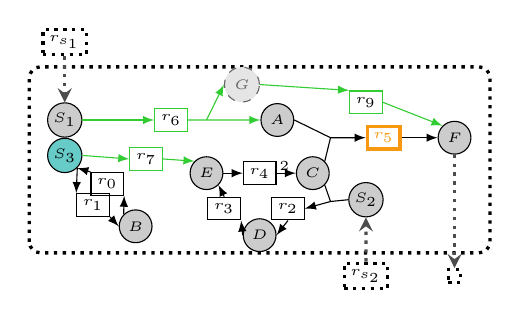
\begin{tikzpicture}[scale=0.45]\tiny
  \tikzstyle{metabolite}=[draw,circle,fill=white!80!black, text width=0.4cm, inner sep=0pt, align=center];
  \tikzstyle{repairmetabolite}=[draw,white!40!black, circle,fill=white!90!black,text=white!40!black,dashed];
  \tikzstyle{seed}=[draw,circle,fill=BlueGreen!70, text width=0.4cm, inner sep=0pt, align=center];%white!80!black
  \tikzstyle{target}=[draw,circle,fill=YellowOrange];%white!40!black
  \tikzstyle{reaction}=[draw,rectangle];
   \tikzstyle{export}=[draw,rectangle,dotted, very thick];
   \tikzstyle{exportrepair}=[draw,rectangle,dotted, very thick,white!80!black,text=white!70!black];
  \tikzstyle{repairreaction}=[draw,rectangle,white!40!black,text=white!40!black,dashed];
  \tikzstyle{solreaction}=[draw,rectangle,LimeGreen,text=black];
  \tikzstyle{initial}=[->,>=latex,thick];
  \tikzstyle{bdd}=[->,>=latex,thick];
  \tikzstyle{etiq}=[midway,fill=black!20,scale=0.5];
  \tikzstyle{stc}=[draw, rectangle, white, text=black]

  \node[stc] (stcr4C) at (6.2,6.7) {$2$};

  \draw [black,dotted, rounded corners, very thick] (-1,4.25) rectangle (12,9.5);
 % \node (system) [draw, rounded rectangle] at (0,0) {} (7cm,5cm);

  \node[seed] (S2) at (0,7) {$S_{3}$};
  \node[metabolite] (Sb2) at (8.5,5.75) {$S_{2}$};
  \node[metabolite] (S1) at (0,8) {$S_{1}$};

  \node[metabolite] (F) at (11,7.50) {$F$};

  \node[metabolite] (A) at (6,8) {$A$};
  \node[metabolite] (B) at (2,5.0) {$B$};
  \node[metabolite] (C) at (7,6.5) {$C$};
  \node[metabolite] (D) at (5.50,4.75) {$D$};
  \node[metabolite] (E) at (4,6.5) {$E$};
  \node[repairmetabolite] (X) at (5,9) {$G$};

  \node[reaction] (R0) at (1.2,6.2) {$r_{0}$};
  \node[reaction] (R1) at (0.8,5.60) {$r_{1}$};
  \node[reaction] (R2) at (6.3,5.5) {$r_{2}$};
  \node[reaction] (R3) at (4.5,5.5) {$r_{3}$};
  \node[reaction] (R4) at (5.5,6.5) {$r_{4}$};
  \node[reaction, very thick,YellowOrange] (R5) at (9,7.50) {$r_{5}$}; %LimeGreen
  \node[solreaction] (R6) at (3,8) {$r_{6}$};
  \node[solreaction] (R7) at (2.3,6.9) {$r_{7}$};
  % \node[repairreaction] (R8) at (3,5.8) {$r_{8}$};
  \node[solreaction] (R9) at (8.5,8.5) {$r_{9}$};

  % R0 : S => B
  \draw[->,>=latex] (B.north west) -- (R0.south east);
  \draw[->,>=latex] (R0.north west) -- (S2.south east);

  % R1 : S <= B
  \draw[->,>=latex] (S2.south east) -- (R1.north west);
  \draw[->,>=latex] (R1.south east) -- (B.west);

  % R2 : Sb2+C => D
  \draw[->,>=latex] (Sb2.west) -- (7.5,5.70) -- (R2.east);
  \draw[] (C.south east) -- (7.5,5.70);
  \draw[->,>=latex] (R2.south) -- (D.east);

  % R3 : D => E
  \draw[->,>=latex] (D.west) -- (R3.south east);
  \draw[->,>=latex] (R3.north) -- (E.south east);

  % R4 : E => C
  \draw[->,>=latex] (E.east) -- (R4.west);
  \draw[->,>=latex] (R4.east) -- (C.west);

  % R5 : A+C => T
  \draw[->,>=latex] (A.east) -- (7.5,7.50) -- (R5.west);
  \draw[] (C.north east) -- (7.5,7.50);
  \draw[->,>=latex] (R5.east) -- (F.west);

  % R6 : S => A+X
  \draw[->,>=latex,LimeGreen] (S1.east) -- (R6.west);
  \draw[->,>=latex,LimeGreen] (R6.east) -- (4,8) -- (A.west);
  \draw[->,>=latex,LimeGreen] (4,8) -- (X.west);

  % R7 : S => E
  \draw[->,>=latex,LimeGreen] (S2.east) -- (R7.west);
  \draw[->,>=latex,LimeGreen] (R7.east) -- (E.north west);
  %
  % % R8 : B => E
  % \draw[->,>=latex,white!55!black,dashed] (B.north east) -- (R8.south west);
  % \draw[->,>=latex,white!55!black,dashed] (R8.east) -- (E.south);

  % R9 : X => F
  \draw[->,>=latex,LimeGreen] (X.east) -- (R9.north west);
  \draw[->,>=latex,LimeGreen] (R9.east) -- (F.north west);

  %export X
  %\node[exportrepair] (outX) at (6.5,10.30) {$r_{expX}$};
  %\draw[->,>=stealth,white!80!black,dotted, very thick] (X.north east) --  (outX.west);

  %export F
  \node[export] (outF) at (11,3.6) {\ExportReaction};
   \draw[->,>=stealth,white!30!black,dotted, very thick] (F.south) --  (outF.north);

  %import S2
   \node[export] (inS) at (0,10.2) {$r_{s_1}$};
   \draw[->,>=stealth,white!30!black,dotted, very thick] (inS.south) --  (S1.north);

   %import Sb2
  \node[export] (inS2) at (8.5,3.6) {$r_{s_2}$};
  \draw[->,>=stealth,white!30!black,dotted, very thick] (inS2) --  (Sb2.south);

\end{tikzpicture}
%
%%% Local Variables:
%%% mode: latex
%%% TeX-master: "paper"
%%% End:

      \caption{First solution to metabolic network completion under hybrid activation hypothesis satisfying Equation~\eqref{eq:hybrid:activation} (that is Equations~\eqref{eq:stoichiometric:bounds},~\eqref{eq:stoichiometric:equation}, ~\eqref{eq:stoichiometric:activation} and ~\eqref{eq:topological:activation}).}
      \label{gra:toy_sh1}
    \end{minipage}%
    \begin{minipage}[t]{.50\textwidth}
      \centering
      %!TEX root = paper.tex
\usetikzlibrary{shapes.misc, positioning}
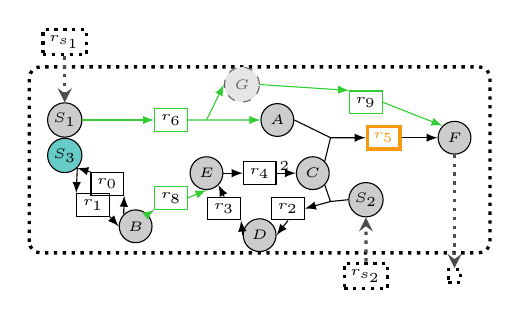
\begin{tikzpicture}[scale=0.45]\tiny
  \tikzstyle{metabolite}=[draw,circle,fill=white!80!black, text width=0.4cm, inner sep=0pt, align=center];
  \tikzstyle{repairmetabolite}=[draw,white!40!black, circle,fill=white!90!black,text=white!40!black,dashed];
  \tikzstyle{seed}=[draw,circle,fill=BlueGreen!70, text width=0.4cm, inner sep=0pt, align=center];%white!80!black
  \tikzstyle{target}=[draw,circle,fill=YellowOrange];%white!40!black
  \tikzstyle{reaction}=[draw,rectangle];
   \tikzstyle{export}=[draw,rectangle,dotted, very thick];
   \tikzstyle{exportrepair}=[draw,rectangle,dotted, very thick,white!80!black,text=white!70!black];
  \tikzstyle{repairreaction}=[draw,rectangle,white!40!black,text=white!40!black,dashed];
  \tikzstyle{solreaction}=[draw,rectangle,LimeGreen,text=black];
  \tikzstyle{initial}=[->,>=latex,thick];
  \tikzstyle{bdd}=[->,>=latex,thick];
  \tikzstyle{etiq}=[midway,fill=black!20,scale=0.5];
  \tikzstyle{stc}=[draw, rectangle, white, text=black]

  \node[stc] (stcr4C) at (6.2,6.7) {$2$};

  \draw [black,dotted, rounded corners, very thick] (-1,4.25) rectangle (12,9.5);
 % \node (system) [draw, rounded rectangle] at (0,0) {} (7cm,5cm);

  \node[seed] (S2) at (0,7) {$S_{3}$};
  \node[metabolite] (Sb2) at (8.5,5.75) {$S_{2}$};
  \node[metabolite] (S1) at (0,8) {$S_{1}$};

  \node[metabolite] (F) at (11,7.50) {$F$};

  \node[metabolite] (A) at (6,8) {$A$};
  \node[metabolite] (B) at (2,5.0) {$B$};
  \node[metabolite] (C) at (7,6.5) {$C$};
  \node[metabolite] (D) at (5.50,4.75) {$D$};
  \node[metabolite] (E) at (4,6.5) {$E$};
  \node[repairmetabolite] (X) at (5,9) {$G$};

  \node[reaction] (R0) at (1.2,6.2) {$r_{0}$};
  \node[reaction] (R1) at (0.8,5.60) {$r_{1}$};
  \node[reaction] (R2) at (6.3,5.5) {$r_{2}$};
  \node[reaction] (R3) at (4.5,5.5) {$r_{3}$};
  \node[reaction] (R4) at (5.5,6.5) {$r_{4}$};
  \node[reaction, very thick,YellowOrange] (R5) at (9,7.50) {$r_{5}$}; %LimeGreen
  \node[solreaction] (R6) at (3,8) {$r_{6}$};
  % \node[solreaction] (R7) at (2.3,6.9) {$r_{7}$};
  \node[solreaction] (R8) at (3,5.8) {$r_{8}$};
  \node[solreaction] (R9) at (8.5,8.5) {$r_{9}$};

  % R0 : S => B
  \draw[->,>=latex] (B.north west) -- (R0.south east);
  \draw[->,>=latex] (R0.north west) -- (S2.south east);

  % R1 : S <= B
  \draw[->,>=latex] (S2.south east) -- (R1.north west);
  \draw[->,>=latex] (R1.south east) -- (B.west);

  % R2 : Sb2+C => D
  \draw[->,>=latex] (Sb2.west) -- (7.5,5.70) -- (R2.east);
  \draw[] (C.south east) -- (7.5,5.70);
  \draw[->,>=latex] (R2.south) -- (D.east);

  % R3 : D => E
  \draw[->,>=latex] (D.west) -- (R3.south east);
  \draw[->,>=latex] (R3.north) -- (E.south east);

  % R4 : E => C
  \draw[->,>=latex] (E.east) -- (R4.west);
  \draw[->,>=latex] (R4.east) -- (C.west);

  % R5 : A+C => T
  \draw[->,>=latex] (A.east) -- (7.5,7.50) -- (R5.west);
  \draw[] (C.north east) -- (7.5,7.50);
  \draw[->,>=latex] (R5.east) -- (F.west);

  % R6 : S => A+X
  \draw[->,>=latex,LimeGreen] (S1.east) -- (R6.west);
  \draw[->,>=latex,LimeGreen] (R6.east) -- (4,8) -- (A.west);
  \draw[->,>=latex,LimeGreen] (4,8) -- (X.west);

  % % R7 : S => E
  % \draw[->,>=latex,white!55!black,dashed] (S2.east) -- (R7.west);
  % \draw[->,>=latex,white!55!black,dashed] (R7.east) -- (E.north west);

  % R8 : B => E
  \draw[->,>=latex,LimeGreen] (B.north east) -- (R8.south west);
  \draw[->,>=latex,LimeGreen] (R8.east) -- (E.south);

  % R9 : X => F
  \draw[->,>=latex,LimeGreen] (X.east) -- (R9.north west);
  \draw[->,>=latex,LimeGreen] (R9.east) -- (F.north west);

  %export X
  %\node[exportrepair] (outX) at (6.5,10.30) {$r_{expX}$};
  %\draw[->,>=stealth,white!80!black,dotted, very thick] (X.north east) --  (outX.west);

  %export F
  \node[export] (outF) at (11,3.6) {\ExportReaction};
   \draw[->,>=stealth,white!30!black,dotted, very thick] (F.south) --  (outF.north);

  %import S2
   \node[export] (inS) at (0,10.2) {$r_{s_1}$};
   \draw[->,>=stealth,white!30!black,dotted, very thick] (inS.south) --  (S1.north);

   %import Sb2
  \node[export] (inS2) at (8.5,3.6) {$r_{s_2}$};
  \draw[->,>=stealth,white!30!black,dotted, very thick] (inS2) --  (Sb2.south);

\end{tikzpicture}
%
%%% Local Variables:
%%% mode: latex
%%% TeX-master: "paper"
%%% End:

      \caption{Second solution to metabolic network completion under hybrid activation hypothesis satisfying Equation~\eqref{eq:hybrid:activation} (that is Equations~\eqref{eq:stoichiometric:bounds},~\eqref{eq:stoichiometric:equation}, ~\eqref{eq:stoichiometric:activation} and ~\eqref{eq:topological:activation}).}
      \label{gra:toy_sh2}
    \end{minipage}
\end{figure}
% ----------------------------------------------------------------------

\subsection{Union of Metabolic Network Completions}\label{sec:union} %emph
As depicted in the toy examples for the topological (Fig.~\ref{gra:toy_st1} and Fig.~\ref{gra:toy_st2}) and hybrid (Fig.~\ref{gra:toy_sh1} and
Fig.~\ref{gra:toy_sh2}) activation, several minimal solutions to one metabolic network completion problem may exist.
There might be dozens of minimal completions, depending on the degradation of the original draft network,
hence leading to difficulties for biologists and bioinformaticians to discriminate the individual results.
One solution to facilitate this curation task is to provide, in addition to the enumeration of solutions, their union.
This has been done previously for the topological completion \citep{Prigent2017}.

% \begin{itemize}
%  \item Since we are able to verify activation for the union of networks,
%        offers us to analyze the quality of approximation methods, like topological and relaxed stoichiometric completion.
%  \item Thus, the idea to union solutions of approximation methods is,
%        to get a may non-minimal set of reactions, which is interesting to may satisfy activation.
% \end{itemize}
Notably, the concept of ``union of solutions" is particularly relevant from the biological perspective since it provides in a single view all possible reactions that could be inserted in a solution to the network completion problem.
%
Additionally, verifying the union according to the desired (stoichiometric and hybrid) activation semantics,
offers a way to analyze the quality of approximation methods (topological and relaxed-stoichiometric ones).
If individual solutions contradict a definition of activation that the union satisfies, it suggests that the family of reactions contained in the union, although possibly non-minimal, may be of interest.
Thus providing merit to the approximation method and their results.

Importantly, we notice that the operation of performing the union of solutions is stable with the concept of activation, although it can contradict the minimality of the size of completion.
Indeed, the union of solutions to the topological network completion problem is itself a (non-minimal) solution to the topological completion problem.
Similarly, the union of minimal stoichiometric solutions always displays the stoichiometric activation of the target reaction(s).
In fact, adding an arbitrary set of reactions to a metabolic network still maintains stoichiometric activation,
since flux distribution for the newly added reactions may be set to zero.
Consequently, the union of minimal hybrid solutions always displays the hybrid activation in the target reaction(s).
%

The following theorems (Theorems ~\ref{th:topo}, ~\ref{th:flux} and ~\ref{th:hybr}) are a formalization of the stability of the union of solutions with respect to the three concepts of activation.


The union $G=G_1\cup G_2$ of two metabolic networks $G_1=(R_1\cup M_1,E_1,\StoichiometricFunction_1)$
and $G_2=(R_2\cup M_2,E_2,\StoichiometricFunction_2)$ is defined by
\begin{align}
G &= (R\cup M, E, \StoichiometricFunction), \label{eq:graph.union1}\\
R &= R_1\cup R_2, \label{eq:graph.union2}\\
M &= M_1\cup M_2, \label{eq:graph.union3}\\
E &= E_1\cup E_2, \label{eq:graph.union4}\\
\StoichiometricFunction &= \StoichiometricFunction_1\cup \StoichiometricFunction_2. \label{eq:graph.union5}
\end{align}

\begin{theorem}\label{th:topo}
Let $G_1$ and $G_2$ be metabolic networks.
If $R_T\subseteq\Activity{t}{G_1}{S}$, then $R_T\subseteq\Activity{t}{G_1\cup G_2}{S}$.
\end{theorem}

\begin{proof}
The proof is given by monotonicity of the union and the monotonicity of the closure.
Thus it can never be case that having more reactions disables reachability.
More formal,
$R_T\subseteq\Activity{t}{G_1}{S}$ holds iff
$\Reactants{r_T}\subseteq\Sigma_{G_1}(S)$.
Furthermore, we have
$\Sigma_{G_1}(S)\subseteq \Sigma_{G_1\cup G_2}(S)$
by the definition of the closure.
This implies
$\Reactants{r_T}\subseteq\Sigma_{G_1\cup G_2}(S)$.
Finally, we have
$R_T\subseteq\Activity{t}{G_1\cup G_2}{S}$.
\end{proof}


\begin{theorem}\label{th:flux}
Let $G_1$ and $G_2$ be metabolic networks.
If $R_T\subseteq\Activity{s}{G_1}{S}$, then $R_T\subseteq\Activity{s}{G_1\cup G_2}{S}$.
\end{theorem}

\begin{proof}
First, we define following bijective functions
\begin{align*}
f:&R_1 \rightarrow \{1,\dots,l\}\subseteq\mathbb{N}, \\
& r \mapsto f(r)=i \\
g:&M_1 \rightarrow \{1,\dots,k\}\subseteq\mathbb{N}, \\
& m \mapsto g(m)=j \\
f':&R_1\cup R_2 \rightarrow \{1,\dots,l'\}\subseteq\mathbb{N}, \\
& r \mapsto f'(r)=
    \begin{cases}
    f(r) &, \text{ if $f(r)$ is defined} \\
    i    &, \text{ otherwise}
    \end{cases} \\
g'&:M_1\cup M_2 \rightarrow \{1,\dots,k'\}\subseteq\mathbb{N} \\
& m \mapsto g'(m)=
    \begin{cases}
    g(m) &, \text{ if $g(m)$ is defined} \\
    j    &, \text{ otherwise}
    \end{cases}
\end{align*}
for $k=|M_1|$, $l=|R_1|$, $k'=|M_1\cup M_2|$ and $l'=|R_1\cup R_2|$ regarding $G_1$ and $G_1\cup G_2$, respectively.
Now, we rewrite the system of (\ref{eq:stoichiometric:equation}) regarding $G_1$ as a matrix equation $Av=0$ of form
\begin{align*}
\begin{pmatrix}
a_{11} & \dots & a_{1l} \\
\vdots & \ddots & \vdots \\
a_{k1} & \dots & a_{kl}
\end{pmatrix}
\begin{pmatrix}
v_1 \\
\vdots  \\
v_l
\end{pmatrix}
=
\begin{pmatrix}
0 \\
\vdots \\
0
\end{pmatrix}\label{eq:matrix}
\end{align*}
where $A$ is a $k\times l$ matrix with coefficients
\begin{align*}
%h: & M_1\times R_1 \rightarrow \mathbb{R} \\
%& (m,r) \mapsto h(m,r)=
a_{g(m)f(r)}=
    \begin{cases}
    \StoichiometricFunction_1(r,m)  &, (r,m)\in E_1 \\
    -\StoichiometricFunction_1(m,r) &, (m,r)\in E_1 \\
    0       &, \text{ otherwise}
    \end{cases}
\end{align*}
and $v$ consists of variables $v_{f(r)}$ for $r\in R_1$.
By $L=\{v\mid Av=0\}$ we denote the set of solutions induced by $Av=0$.

Furthermore, we represent the system of linear equations of (\ref{eq:stoichiometric:equation}) regarding $G_1\cup G_2$ as a matrix equation $A'v'=0$ of form
\begin{align*}
\begin{pmatrix}
a_{11} & \dots & a_{1l} & a_{1l+1} & \dots & a_{1l'} \\
\vdots & \ddots& \vdots & \vdots   & \ddots& \vdots \\
a_{k1} & \dots & a_{kl} & a_{kl+1} & \dots & a_{kl'} \\
0      & \dots & 0      & a_{k+1l+1} & \dots & a_{k+1l'} \\
\vdots & \ddots& \vdots & \vdots   & \ddots& \vdots \\
0      & \dots & 0      & a_{k'l+1}& \dots & a_{k'l'}
\end{pmatrix}
\begin{pmatrix}
v_1 \\
\vdots  \\
v_l \\
v_{l+1} \\
\vdots \\
v_{l'}
\end{pmatrix}
=
\begin{pmatrix}
0 \\
\vdots \\
0
\end{pmatrix}%\label{eq:matrix2}
\end{align*}
where $A'$ is a $k'\times l'$ matrix with coefficients
\begin{align*}
% h': & (M_1\cup M_2)\times(R_1\cup R_2) \rightarrow \mathbb{R} \\
%& (m,r) \mapsto h'(m,r)=
a_{g'(m)f'(r)}=
    \begin{cases}
    \StoichiometricFunction(r,m)  &, (r,m)\in E_1\cup E_2 \\
    -\StoichiometricFunction(m,r) &, (m,r)\in E_1\cup E_2 \\
    0       &, \text{ otherwise}
    \end{cases}
\end{align*}
where $\StoichiometricFunction=\StoichiometricFunction_1\cup \StoichiometricFunction_2$
and $v'$ consists of variables $v_{f'(r)}$ of (\ref{eq:stoichiometric:equation}) for $r\in R_1\cup R_2$.
Note that $A'$ can always be written in this form, since switching columns and rows will not change solutions.
By $L'=\{v'\mid A'v'=0\}$ we denote the set of solutions induced by $A'v'=0$.

Since $A'v'=0$ is homogeneous, $L\subseteq L'$ holds by extending $L$ with zeros for $v_{f'(r)}$ with $r\in R_2\setminus R_1$.
Thus $\{v\mid v\in L, \forall r_T\in R_T, v_{f(r_T)}>0\}
\subseteq\{v\mid v\in L', \forall r_T\in R_T, v_{f'(r_T)}>0\}$
by extending the first set with zeros for $v_{f'(r)}$ with $r\in R_2\setminus R_1$.
From $R_T\subseteq\Activity{s}{G_1}{S}$, we know that the homogeneous system of linear equations from
(\ref{eq:stoichiometric:equation}) regarding $G_1$ is non-trivial satisfiable,
which finally implies that $R_T\subseteq\Activity{s}{G_1\cup G_2}{S}$.
\end{proof}


\begin{theorem}\label{th:hybr}
Let $G_1$ and $G_2$ be metabolic networks.
If $R_T\subseteq\Activity{h}{G_1}{S}$, then $R_T\subseteq\Activity{h}{G_1\cup G_2}{S}$.
\end{theorem}

\begin{proof}
Follows directly by the definition of hybrid activation together with Theorem~\ref{th:topo} and Theorem~\ref{th:flux}.
More formal,
$R_T\subseteq\Activity{h}{G_1}{S}$
holds iff
$R_T\subseteq\Activity{t}{G_1}{S}$ and $R_T\subseteq\Activity{s}{G_1}{S}$.
From Theorem~\ref{th:topo} and $R_T\subseteq\Activity{t}{G_1}{S}$ follows
$R_T\subseteq\Activity{t}{G_1\cup G_2}{S}$.
Analogously, from Theorem~\ref{th:flux} and $R_T\subseteq\Activity{s}{G_1}{S}$ follows
$R_T\subseteq\Activity{s}{G_1\cup G_2}{S}$.
Finally, this implies
$R_T\subseteq\Activity{h}{G_1\cup G_2}{S}$.
\end{proof}



In particular, studying the union in case of topological modeling can pinpoint interesting cases.
Individual solutions satisfying the topological activation can additionally satisfy the stoichiometric and thus the hybrid activation semantics.
A union including such a solution will also adhere to the hybrid standard.
In some cases, the union of solutions will display the stoichiometric activation whereas the individual solutions only satisfy the topological activation.
Fig.~\ref{gra:union_nf_f1} to Fig.~\ref{gra:union_nf_f} display an example of topological metabolic network completions that do not satisfy stoichiometric (and hybrid) activation whereas their union does.
Fig.~\ref{gra:union_nf_nf1} to Fig.~\ref{gra:union_nf_nf} provide an example of minimal topological completions that do not satisfy stoichiometric (and hybrid) activation and for which the union does not satisfy it either.
%
%Both observations induce that in general we cannot derive anything about activation of reactions for an unionized graph if both of the previous graphs do not satisfy activation of these reactions as well.


Both observations induce that in general we cannot derive anything about activation of reactions in a graph resulting from the union of two or more graphs.
And similarly, we cannot infer about the activation of reactions in subgraphs arbitrarily derived from a graph in which these reactions are activated.


% ----------------------------------------------------------------------
\begin{figure}
    \captionsetup{width=0.3\textwidth}
    \centering
    \begin{minipage}[t]{.32\textwidth}
      % \documentclass{article}
% \usepackage[dvipsnames]{xcolor}
% \usepackage{tikz}
% \usepackage{xcolor,colortbl}
% 
% \begin{document}
% 
% \newcommand{\gringo}{\textit{gringo}}
\newcommand{\clasp}{\textit{clasp}}
\newcommand{\clingo}{\textit{clingo}}
\newcommand{\asprin}{\textit{asprin}}
\newcommand{\asap}{\textit{teaspoon}}
\newcommand{\piclasp}{\textit{piclasp}}

\newcommand{\code}[1]{\lstinline[basicstyle=\ttfamily]{#1}}

\newcommand{\lw}[1]{\smash{\lower1.ex\hbox{#1}}}
\newcommand{\llw}[1]{\smash{\lower3.ex\hbox{#1}}}

%\newcommand{\dataCL}[5]{%
%  \code{#1} & #3 & #5 & #4
%}
%\newcommand{\dataCS}[5]{%
%  #3 & #5 & #4
%}

\newenvironment{tableC}{%
  \scriptsize
  \tabcolsep = 0.6mm
  \begin{tabular}[t]{l|rlr|rlr|rlr|rlr|rlr}\hline
    \multicolumn{1}{l|}{\llw{Instance}} &
    \multicolumn{3}{c|}{UD1} &
    \multicolumn{3}{c|}{UD2} &
    \multicolumn{3}{c|}{UD3} &
    \multicolumn{3}{c|}{UD4} &
    \multicolumn{3}{c}{UD5} \\
    & 
    \multicolumn{1}{c}{Best} & & \multicolumn{1}{c|}{\emph{tea-}} & 
    \multicolumn{1}{c}{Best} & & \multicolumn{1}{c|}{\emph{tea-}} & 
    \multicolumn{1}{c}{Best} & & \multicolumn{1}{c|}{\emph{tea-}} & 
    \multicolumn{1}{c}{Best} & & \multicolumn{1}{c|}{\emph{tea-}} & 
    \multicolumn{1}{c}{Best} & & \multicolumn{1}{c}{\emph{tea-}} \\
    & 
    known & & \emph{spoon} & 
    known & & \emph{spoon} & 
    known & & \emph{spoon} & 
    known & & \emph{spoon} & 
    known & & \emph{spoon} \\
    \hline
  }{%
    \hline
  \end{tabular}
}

\newenvironment{tableB}{%
  \scriptsize
  \tabcolsep = 0.7mm
%  \begin{tabular}[t]{|l|c|r|l|l|l|}\hline
  \begin{tabular}[t]{lcrlll}\hline
    Instance &
    Formulation &
    Time (sec.)\\
    \hline
  }{%
    \hline
  \end{tabular}
}
\newenvironment{tableL}{%
  \scriptsize
  \tabcolsep = 0.7mm
  \begin{tabular}[t]{l|rrrrrrrr|r}\hline
    \lw{Instance} &
    \lw{Time (sec.)} &
    \multicolumn{6}{c}{The best utility vector} &
    The sum of  &
    The best of basic\\
    &
    &
    $(S_1,$ & $S_4,$ & $S_2,$ & $S_7,$ & $S_6,$ & $S_3)$ &
    utility vector &
    and optimized \\
    \hline
  }{%
    \hline
  \end{tabular}
}

%%% Local Variables:
%%% mode: latex
%%% TeX-master: "paper"
%%% End:


% \begin{figure}[t]
%   \centering

    \usetikzlibrary{shapes.misc, positioning}
    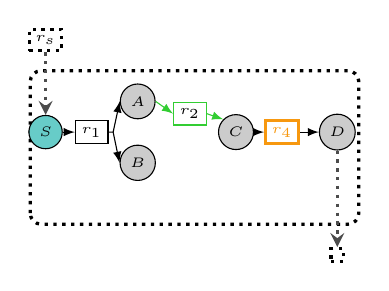
\begin{tikzpicture}[scale=0.39]\tiny
      \tikzstyle{metabolite}=[draw,circle,fill=white!80!black];
      \tikzstyle{repairmetabolite}=[draw,white!40!black, circle,fill=white!90!black,text=white!40!black,dashed];
      \tikzstyle{seed}=[draw,circle,fill=BlueGreen!70];%white!80!black
      \tikzstyle{target}=[draw,circle,fill=YellowOrange];%white!40!black
      \tikzstyle{reaction}=[draw,rectangle];
       \tikzstyle{export}=[draw,rectangle,dotted, very thick];
       \tikzstyle{exportrepair}=[draw,rectangle,dotted, very thick,white!80!black,text=white!70!black];
      \tikzstyle{repairreaction}=[draw,rectangle,white!40!black,text=white!40!black,dashed];
      \tikzstyle{solreaction}=[draw,rectangle,LimeGreen,text=black];
      \tikzstyle{initial}=[->,>=latex,thick];
      \tikzstyle{bdd}=[->,>=latex,thick];
      \tikzstyle{etiq}=[midway,fill=black!20,scale=0.5];
      \tikzstyle{stc}=[draw, rectangle, white, text=black]


      \draw [black,dotted, rounded corners, very thick] (-0.5,4) rectangle (10.2,9);
     % \node (system) [draw, rounded rectangle] at (0,0) {} (7cm,5cm);

      \node[seed] (S) at (0,7) {$S$};
      \node[metabolite] (A) at (3,8) {$A$};
      \node[metabolite] (B) at (3,6) {$B$};
      \node[metabolite] (C) at (6.2,7) {$C$};
      \node[metabolite] (D) at (9.5,7) {$D$};

      \node[reaction] (R1) at (1.5,7) {$r_{1}$};
      \node[reaction, very thick,YellowOrange] (R4) at (7.7,7) {$r_{4}$}; %LimeGreen
      \node[solreaction] (R2) at (4.7,7.6) {$r_{2}$};
      %\node[solreaction] (R3) at (4.7,6.4) {$r_{3}$};

      % R1 : S => A + B
      \draw[->,>=latex] (S.east) -- (R1.west);
      \draw[->,>=latex] (R1.east) -- (2.2,7) -- (A.west);
      \draw[->,>=latex] (2.2,7)  -- (B.west);

      % R2 : A => C
      \draw[->,>=latex,LimeGreen] (A.east) -- (R2.west);
      \draw[->,>=latex,LimeGreen] (R2.east) -- (C.north west);

      % R3 : B => C
      %\draw[->,>=latex,LimeGreen] (B.east) -- (R3.west);
      %\draw[->,>=latex,LimeGreen] (R3.east) -- (C.south west);

      % R4 : C => D
      \draw[->,>=latex] (C.east) -- (R4.west);
      \draw[->,>=latex] (R4.east) -- (D.west);

      %export G
      \node[export] (outD) at (9.5,3) {\ExportReaction};
      \draw[->,>=stealth,white!30!black,dotted, very thick] (D.south) --  (outD.north);

      %import S2
      \node[export] (inS) at (0,10) {$r_{s}$};
      \draw[->,>=stealth,white!30!black,dotted, very thick] (inS) --  (S.north);

  \end{tikzpicture}
% \end{figure}

% \end{document}

      \caption{Topological completion $R_1=\{r_2\}$ satisfies $r_4\in\Activity{t}{G_1}{\{S\}}$, but carries no flux, due to accumulation of compound $B$ that contradicts Eq.~\ref{eq:stoichiometric:equation}.\label{gra:union_nf_f1}}
    \end{minipage}
    \begin{minipage}[t]{.32\textwidth}
      % \documentclass{article}
% \usepackage[dvipsnames]{xcolor}
% \usepackage{tikz}
% \usepackage{xcolor,colortbl}
% 
% \begin{document}
% 
% \newcommand{\gringo}{\textit{gringo}}
\newcommand{\clasp}{\textit{clasp}}
\newcommand{\clingo}{\textit{clingo}}
\newcommand{\asprin}{\textit{asprin}}
\newcommand{\asap}{\textit{teaspoon}}
\newcommand{\piclasp}{\textit{piclasp}}

\newcommand{\code}[1]{\lstinline[basicstyle=\ttfamily]{#1}}

\newcommand{\lw}[1]{\smash{\lower1.ex\hbox{#1}}}
\newcommand{\llw}[1]{\smash{\lower3.ex\hbox{#1}}}

%\newcommand{\dataCL}[5]{%
%  \code{#1} & #3 & #5 & #4
%}
%\newcommand{\dataCS}[5]{%
%  #3 & #5 & #4
%}

\newenvironment{tableC}{%
  \scriptsize
  \tabcolsep = 0.6mm
  \begin{tabular}[t]{l|rlr|rlr|rlr|rlr|rlr}\hline
    \multicolumn{1}{l|}{\llw{Instance}} &
    \multicolumn{3}{c|}{UD1} &
    \multicolumn{3}{c|}{UD2} &
    \multicolumn{3}{c|}{UD3} &
    \multicolumn{3}{c|}{UD4} &
    \multicolumn{3}{c}{UD5} \\
    & 
    \multicolumn{1}{c}{Best} & & \multicolumn{1}{c|}{\emph{tea-}} & 
    \multicolumn{1}{c}{Best} & & \multicolumn{1}{c|}{\emph{tea-}} & 
    \multicolumn{1}{c}{Best} & & \multicolumn{1}{c|}{\emph{tea-}} & 
    \multicolumn{1}{c}{Best} & & \multicolumn{1}{c|}{\emph{tea-}} & 
    \multicolumn{1}{c}{Best} & & \multicolumn{1}{c}{\emph{tea-}} \\
    & 
    known & & \emph{spoon} & 
    known & & \emph{spoon} & 
    known & & \emph{spoon} & 
    known & & \emph{spoon} & 
    known & & \emph{spoon} \\
    \hline
  }{%
    \hline
  \end{tabular}
}

\newenvironment{tableB}{%
  \scriptsize
  \tabcolsep = 0.7mm
%  \begin{tabular}[t]{|l|c|r|l|l|l|}\hline
  \begin{tabular}[t]{lcrlll}\hline
    Instance &
    Formulation &
    Time (sec.)\\
    \hline
  }{%
    \hline
  \end{tabular}
}
\newenvironment{tableL}{%
  \scriptsize
  \tabcolsep = 0.7mm
  \begin{tabular}[t]{l|rrrrrrrr|r}\hline
    \lw{Instance} &
    \lw{Time (sec.)} &
    \multicolumn{6}{c}{The best utility vector} &
    The sum of  &
    The best of basic\\
    &
    &
    $(S_1,$ & $S_4,$ & $S_2,$ & $S_7,$ & $S_6,$ & $S_3)$ &
    utility vector &
    and optimized \\
    \hline
  }{%
    \hline
  \end{tabular}
}

%%% Local Variables:
%%% mode: latex
%%% TeX-master: "paper"
%%% End:


% \begin{figure}[t]
%   \centering

    \usetikzlibrary{shapes.misc, positioning}
    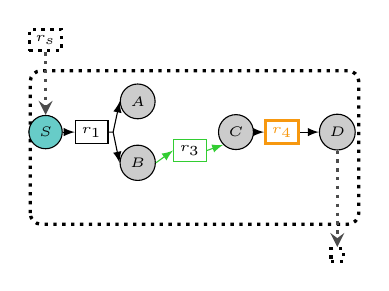
\begin{tikzpicture}[scale=0.39]\tiny
      \tikzstyle{metabolite}=[draw,circle,fill=white!80!black];
      \tikzstyle{repairmetabolite}=[draw,white!40!black, circle,fill=white!90!black,text=white!40!black,dashed];
      \tikzstyle{seed}=[draw,circle,fill=BlueGreen!70];%white!80!black
      \tikzstyle{target}=[draw,circle,fill=YellowOrange];%white!40!black
      \tikzstyle{reaction}=[draw,rectangle];
       \tikzstyle{export}=[draw,rectangle,dotted, very thick];
       \tikzstyle{exportrepair}=[draw,rectangle,dotted, very thick,white!80!black,text=white!70!black];
      \tikzstyle{repairreaction}=[draw,rectangle,white!40!black,text=white!40!black,dashed];
      \tikzstyle{solreaction}=[draw,rectangle,LimeGreen,text=black];
      \tikzstyle{initial}=[->,>=latex,thick];
      \tikzstyle{bdd}=[->,>=latex,thick];
      \tikzstyle{etiq}=[midway,fill=black!20,scale=0.5];
      \tikzstyle{stc}=[draw, rectangle, white, text=black]


      \draw [black,dotted, rounded corners, very thick] (-0.5,4) rectangle (10.2,9);
     % \node (system) [draw, rounded rectangle] at (0,0) {} (7cm,5cm);

      \node[seed] (S) at (0,7) {$S$};
      \node[metabolite] (A) at (3,8) {$A$};
      \node[metabolite] (B) at (3,6) {$B$};
      \node[metabolite] (C) at (6.2,7) {$C$};
      \node[metabolite] (D) at (9.5,7) {$D$};

      \node[reaction] (R1) at (1.5,7) {$r_{1}$};
      \node[reaction, very thick,YellowOrange] (R4) at (7.7,7) {$r_{4}$}; %LimeGreen
      %\node[solreaction] (R2) at (4.7,7.6) {$r_{2}$};
      \node[solreaction] (R3) at (4.7,6.4) {$r_{3}$};

      % R1 : S => A + B
      \draw[->,>=latex] (S.east) -- (R1.west);
      \draw[->,>=latex] (R1.east) -- (2.2,7) -- (A.west);
      \draw[->,>=latex] (2.2,7)  -- (B.west);

      % R2 : A => C
      %\draw[->,>=latex,LimeGreen] (A.east) -- (R2.west);
      %\draw[->,>=latex,LimeGreen] (R2.east) -- (C.north west);

      % R3 : B => C
      \draw[->,>=latex,LimeGreen] (B.east) -- (R3.west);
      \draw[->,>=latex,LimeGreen] (R3.east) -- (C.south west);

      % R4 : C => D
      \draw[->,>=latex] (C.east) -- (R4.west);
      \draw[->,>=latex] (R4.east) -- (D.west);

      %export G
      \node[export] (outD) at (9.5,3) {\ExportReaction};
      \draw[->,>=stealth,white!30!black,dotted, very thick] (D.south) --  (outD.north);

      %import S2
      \node[export] (inS) at (0,10) {$r_{s}$};
      \draw[->,>=stealth,white!30!black,dotted, very thick] (inS) --  (S.north);

  \end{tikzpicture}
% \end{figure}

% \end{document}

      \caption{Topological completion $R_2=\{r_3\}$ satisfies $r_4\in\Activity{t}{G_2}{\{S\}}$ and carries no flux as well, due to accumulation of compound $A$ that contradicts Eq.~\ref{eq:stoichiometric:equation}.\label{gra:union_nf_f2}}
    \end{minipage}
    \begin{minipage}[t]{.32\textwidth}
      % \documentclass{article}
% \usepackage[dvipsnames]{xcolor}
% \usepackage{tikz}
% \usepackage{xcolor,colortbl}
% 
% \begin{document}
% 
% \newcommand{\gringo}{\textit{gringo}}
\newcommand{\clasp}{\textit{clasp}}
\newcommand{\clingo}{\textit{clingo}}
\newcommand{\asprin}{\textit{asprin}}
\newcommand{\asap}{\textit{teaspoon}}
\newcommand{\piclasp}{\textit{piclasp}}

\newcommand{\code}[1]{\lstinline[basicstyle=\ttfamily]{#1}}

\newcommand{\lw}[1]{\smash{\lower1.ex\hbox{#1}}}
\newcommand{\llw}[1]{\smash{\lower3.ex\hbox{#1}}}

%\newcommand{\dataCL}[5]{%
%  \code{#1} & #3 & #5 & #4
%}
%\newcommand{\dataCS}[5]{%
%  #3 & #5 & #4
%}

\newenvironment{tableC}{%
  \scriptsize
  \tabcolsep = 0.6mm
  \begin{tabular}[t]{l|rlr|rlr|rlr|rlr|rlr}\hline
    \multicolumn{1}{l|}{\llw{Instance}} &
    \multicolumn{3}{c|}{UD1} &
    \multicolumn{3}{c|}{UD2} &
    \multicolumn{3}{c|}{UD3} &
    \multicolumn{3}{c|}{UD4} &
    \multicolumn{3}{c}{UD5} \\
    & 
    \multicolumn{1}{c}{Best} & & \multicolumn{1}{c|}{\emph{tea-}} & 
    \multicolumn{1}{c}{Best} & & \multicolumn{1}{c|}{\emph{tea-}} & 
    \multicolumn{1}{c}{Best} & & \multicolumn{1}{c|}{\emph{tea-}} & 
    \multicolumn{1}{c}{Best} & & \multicolumn{1}{c|}{\emph{tea-}} & 
    \multicolumn{1}{c}{Best} & & \multicolumn{1}{c}{\emph{tea-}} \\
    & 
    known & & \emph{spoon} & 
    known & & \emph{spoon} & 
    known & & \emph{spoon} & 
    known & & \emph{spoon} & 
    known & & \emph{spoon} \\
    \hline
  }{%
    \hline
  \end{tabular}
}

\newenvironment{tableB}{%
  \scriptsize
  \tabcolsep = 0.7mm
%  \begin{tabular}[t]{|l|c|r|l|l|l|}\hline
  \begin{tabular}[t]{lcrlll}\hline
    Instance &
    Formulation &
    Time (sec.)\\
    \hline
  }{%
    \hline
  \end{tabular}
}
\newenvironment{tableL}{%
  \scriptsize
  \tabcolsep = 0.7mm
  \begin{tabular}[t]{l|rrrrrrrr|r}\hline
    \lw{Instance} &
    \lw{Time (sec.)} &
    \multicolumn{6}{c}{The best utility vector} &
    The sum of  &
    The best of basic\\
    &
    &
    $(S_1,$ & $S_4,$ & $S_2,$ & $S_7,$ & $S_6,$ & $S_3)$ &
    utility vector &
    and optimized \\
    \hline
  }{%
    \hline
  \end{tabular}
}

%%% Local Variables:
%%% mode: latex
%%% TeX-master: "paper"
%%% End:


% \begin{figure}[t]
%   \centering

    \usetikzlibrary{shapes.misc, positioning}
    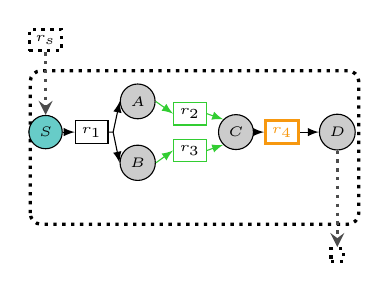
\begin{tikzpicture}[scale=0.39]\tiny
      \tikzstyle{metabolite}=[draw,circle,fill=white!80!black];
      \tikzstyle{repairmetabolite}=[draw,white!40!black, circle,fill=white!90!black,text=white!40!black,dashed];
      \tikzstyle{seed}=[draw,circle,fill=BlueGreen!70];%white!80!black
      \tikzstyle{target}=[draw,circle,fill=YellowOrange];%white!40!black
      \tikzstyle{reaction}=[draw,rectangle];
       \tikzstyle{export}=[draw,rectangle,dotted, very thick];
       \tikzstyle{exportrepair}=[draw,rectangle,dotted, very thick,white!80!black,text=white!70!black];
      \tikzstyle{repairreaction}=[draw,rectangle,white!40!black,text=white!40!black,dashed];
      \tikzstyle{solreaction}=[draw,rectangle,LimeGreen,text=black];
      \tikzstyle{initial}=[->,>=latex,thick];
      \tikzstyle{bdd}=[->,>=latex,thick];
      \tikzstyle{etiq}=[midway,fill=black!20,scale=0.5];
      \tikzstyle{stc}=[draw, rectangle, white, text=black]


      \draw [black,dotted, rounded corners, very thick] (-0.5,4) rectangle (10.2,9);
     % \node (system) [draw, rounded rectangle] at (0,0) {} (7cm,5cm);

      \node[seed] (S) at (0,7) {$S$};
      \node[metabolite] (A) at (3,8) {$A$};
      \node[metabolite] (B) at (3,6) {$B$};
      \node[metabolite] (C) at (6.2,7) {$C$};
      \node[metabolite] (D) at (9.5,7) {$D$};

      \node[reaction] (R1) at (1.5,7) {$r_{1}$};
      \node[reaction, very thick,YellowOrange] (R4) at (7.7,7) {$r_{4}$}; %LimeGreen
      \node[solreaction] (R2) at (4.7,7.6) {$r_{2}$};
      \node[solreaction] (R3) at (4.7,6.4) {$r_{3}$};

      % R1 : S => A + B
      \draw[->,>=latex] (S.east) -- (R1.west);
      \draw[->,>=latex] (R1.east) -- (2.2,7) -- (A.west);
      \draw[->,>=latex] (2.2,7)  -- (B.west);

      % R2 : A => C
      \draw[->,>=latex,LimeGreen] (A.east) -- (R2.west);
      \draw[->,>=latex,LimeGreen] (R2.east) -- (C.north west);

      % R3 : B => C
      \draw[->,>=latex,LimeGreen] (B.east) -- (R3.west);
      \draw[->,>=latex,LimeGreen] (R3.east) -- (C.south west);

      % R4 : C => D
      \draw[->,>=latex] (C.east) -- (R4.west);
      \draw[->,>=latex] (R4.east) -- (D.west);

      %export G
      \node[export] (outD) at (9.5,3) {\ExportReaction};
      \draw[->,>=stealth,white!30!black,dotted, very thick] (D.south) --  (outD.north);

      %import S2
      \node[export] (inS) at (0,10) {$r_{s}$};
      \draw[->,>=stealth,white!30!black,dotted, very thick] (inS) --  (S.north);

  \end{tikzpicture}
% \end{figure}

% \end{document}

      \caption{Completion with the union $R_1\cup R_2=\{r_2,r_3\}$. $G=G_1\cup G_2$  satisfies $r_4\in\Activity{h}{G}{\{S\}}$ and thus is flux-balanced.
      \label{gra:union_nf_f}}
    \end{minipage}
\end{figure}
% ----------------------------------------------------------------------


% ----------------------------------------------------------------------
\begin{figure}
    \captionsetup{width=0.3\textwidth}
    \centering
    \begin{minipage}[t]{.32\textwidth}
      % \documentclass{article}
% \usepackage[dvipsnames]{xcolor}
% \usepackage{tikz}
% \usepackage{xcolor,colortbl}
% 
% \begin{document}
% 
% \newcommand{\gringo}{\textit{gringo}}
\newcommand{\clasp}{\textit{clasp}}
\newcommand{\clingo}{\textit{clingo}}
\newcommand{\asprin}{\textit{asprin}}
\newcommand{\asap}{\textit{teaspoon}}
\newcommand{\piclasp}{\textit{piclasp}}

\newcommand{\code}[1]{\lstinline[basicstyle=\ttfamily]{#1}}

\newcommand{\lw}[1]{\smash{\lower1.ex\hbox{#1}}}
\newcommand{\llw}[1]{\smash{\lower3.ex\hbox{#1}}}

%\newcommand{\dataCL}[5]{%
%  \code{#1} & #3 & #5 & #4
%}
%\newcommand{\dataCS}[5]{%
%  #3 & #5 & #4
%}

\newenvironment{tableC}{%
  \scriptsize
  \tabcolsep = 0.6mm
  \begin{tabular}[t]{l|rlr|rlr|rlr|rlr|rlr}\hline
    \multicolumn{1}{l|}{\llw{Instance}} &
    \multicolumn{3}{c|}{UD1} &
    \multicolumn{3}{c|}{UD2} &
    \multicolumn{3}{c|}{UD3} &
    \multicolumn{3}{c|}{UD4} &
    \multicolumn{3}{c}{UD5} \\
    & 
    \multicolumn{1}{c}{Best} & & \multicolumn{1}{c|}{\emph{tea-}} & 
    \multicolumn{1}{c}{Best} & & \multicolumn{1}{c|}{\emph{tea-}} & 
    \multicolumn{1}{c}{Best} & & \multicolumn{1}{c|}{\emph{tea-}} & 
    \multicolumn{1}{c}{Best} & & \multicolumn{1}{c|}{\emph{tea-}} & 
    \multicolumn{1}{c}{Best} & & \multicolumn{1}{c}{\emph{tea-}} \\
    & 
    known & & \emph{spoon} & 
    known & & \emph{spoon} & 
    known & & \emph{spoon} & 
    known & & \emph{spoon} & 
    known & & \emph{spoon} \\
    \hline
  }{%
    \hline
  \end{tabular}
}

\newenvironment{tableB}{%
  \scriptsize
  \tabcolsep = 0.7mm
%  \begin{tabular}[t]{|l|c|r|l|l|l|}\hline
  \begin{tabular}[t]{lcrlll}\hline
    Instance &
    Formulation &
    Time (sec.)\\
    \hline
  }{%
    \hline
  \end{tabular}
}
\newenvironment{tableL}{%
  \scriptsize
  \tabcolsep = 0.7mm
  \begin{tabular}[t]{l|rrrrrrrr|r}\hline
    \lw{Instance} &
    \lw{Time (sec.)} &
    \multicolumn{6}{c}{The best utility vector} &
    The sum of  &
    The best of basic\\
    &
    &
    $(S_1,$ & $S_4,$ & $S_2,$ & $S_7,$ & $S_6,$ & $S_3)$ &
    utility vector &
    and optimized \\
    \hline
  }{%
    \hline
  \end{tabular}
}

%%% Local Variables:
%%% mode: latex
%%% TeX-master: "paper"
%%% End:


% \begin{figure}[t]
%   \centering

    \usetikzlibrary{shapes.misc, positioning}
    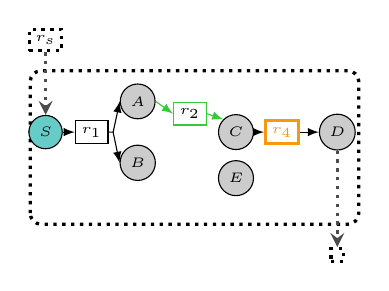
\begin{tikzpicture}[scale=0.39]\tiny
      \tikzstyle{metabolite}=[draw,circle,fill=white!80!black];
      \tikzstyle{repairmetabolite}=[draw,white!40!black, circle,fill=white!90!black,text=white!40!black,dashed];
      \tikzstyle{seed}=[draw,circle,fill=BlueGreen!70];%white!80!black
      \tikzstyle{target}=[draw,circle,fill=YellowOrange];%white!40!black
      \tikzstyle{reaction}=[draw,rectangle];
       \tikzstyle{export}=[draw,rectangle,dotted, very thick];
       \tikzstyle{exportrepair}=[draw,rectangle,dotted, very thick,white!80!black,text=white!70!black];
      \tikzstyle{repairreaction}=[draw,rectangle,white!40!black,text=white!40!black,dashed];
      \tikzstyle{solreaction}=[draw,rectangle,LimeGreen,text=black];
      \tikzstyle{initial}=[->,>=latex,thick];
      \tikzstyle{bdd}=[->,>=latex,thick];
      \tikzstyle{etiq}=[midway,fill=black!20,scale=0.5];
      \tikzstyle{stc}=[draw, rectangle, white, text=black]


      \draw [black,dotted, rounded corners, very thick] (-0.5,4) rectangle (10.2,9);
     % \node (system) [draw, rounded rectangle] at (0,0) {} (7cm,5cm);

      \node[seed] (S) at (0,7) {$S$};
      \node[metabolite] (A) at (3,8) {$A$};
      \node[metabolite] (B) at (3,6) {$B$};
      \node[metabolite] (C) at (6.2,7) {$C$};
      \node[metabolite] (D) at (9.5,7) {$D$};
      \node[metabolite] (E) at (6.2,5.5) {$E$};

      \node[reaction] (R1) at (1.5,7) {$r_{1}$};
      \node[reaction, very thick,YellowOrange] (R4) at (7.7,7) {$r_{4}$}; %LimeGreen
      \node[solreaction] (R2) at (4.7,7.6) {$r_{2}$};
      %\node[solreaction] (R3) at (4.7,6.4) {$r_{3}$};

      % R1 : S => A + B
      \draw[->,>=latex] (S.east) -- (R1.west);
      \draw[->,>=latex] (R1.east) -- (2.2,7) -- (A.west);
      \draw[->,>=latex] (2.2,7)  -- (B.west);

      % R2 : A => C
      \draw[->,>=latex,LimeGreen] (A.east) -- (R2.west);
      \draw[->,>=latex,LimeGreen] (R2.east) -- (C.north west);

      % R3 : B => C + E
      %\draw[->,>=latex,LimeGreen] (B.east) -- (R3.west);
      %\draw[->,>=latex,LimeGreen] (R3.east) -- (C.south west);
      %\draw[->,>=latex,LimeGreen] (R3.east) -- (E.west);

      % R4 : C => D
      \draw[->,>=latex] (C.east) -- (R4.west);
      \draw[->,>=latex] (R4.east) -- (D.west);

      %export G
      \node[export] (outD) at (9.5,3) {\ExportReaction};
      \draw[->,>=stealth,white!30!black,dotted, very thick] (D.south) --  (outD.north);

      %import S2
      \node[export] (inS) at (0,10) {$r_{s}$};
      \draw[->,>=stealth,white!30!black,dotted, very thick] (inS) --  (S.north);

  \end{tikzpicture}
% \end{figure}

% \end{document}

      \caption{Topological completion $R_1=\{r_2\}$ satisfies $r_4\in\Activity{t}{G_1}{\{S\}}$, but carries no flux, due to accumulation of compound $B$ that contradicts Eq.~\ref{eq:stoichiometric:equation}.\label{gra:union_nf_nf1}}
    \end{minipage}
    \begin{minipage}[t]{.32\textwidth}
      % \documentclass{article}
% \usepackage[dvipsnames]{xcolor}
% \usepackage{tikz}
% \usepackage{xcolor,colortbl}
% 
% \begin{document}
% 
% \newcommand{\gringo}{\textit{gringo}}
\newcommand{\clasp}{\textit{clasp}}
\newcommand{\clingo}{\textit{clingo}}
\newcommand{\asprin}{\textit{asprin}}
\newcommand{\asap}{\textit{teaspoon}}
\newcommand{\piclasp}{\textit{piclasp}}

\newcommand{\code}[1]{\lstinline[basicstyle=\ttfamily]{#1}}

\newcommand{\lw}[1]{\smash{\lower1.ex\hbox{#1}}}
\newcommand{\llw}[1]{\smash{\lower3.ex\hbox{#1}}}

%\newcommand{\dataCL}[5]{%
%  \code{#1} & #3 & #5 & #4
%}
%\newcommand{\dataCS}[5]{%
%  #3 & #5 & #4
%}

\newenvironment{tableC}{%
  \scriptsize
  \tabcolsep = 0.6mm
  \begin{tabular}[t]{l|rlr|rlr|rlr|rlr|rlr}\hline
    \multicolumn{1}{l|}{\llw{Instance}} &
    \multicolumn{3}{c|}{UD1} &
    \multicolumn{3}{c|}{UD2} &
    \multicolumn{3}{c|}{UD3} &
    \multicolumn{3}{c|}{UD4} &
    \multicolumn{3}{c}{UD5} \\
    & 
    \multicolumn{1}{c}{Best} & & \multicolumn{1}{c|}{\emph{tea-}} & 
    \multicolumn{1}{c}{Best} & & \multicolumn{1}{c|}{\emph{tea-}} & 
    \multicolumn{1}{c}{Best} & & \multicolumn{1}{c|}{\emph{tea-}} & 
    \multicolumn{1}{c}{Best} & & \multicolumn{1}{c|}{\emph{tea-}} & 
    \multicolumn{1}{c}{Best} & & \multicolumn{1}{c}{\emph{tea-}} \\
    & 
    known & & \emph{spoon} & 
    known & & \emph{spoon} & 
    known & & \emph{spoon} & 
    known & & \emph{spoon} & 
    known & & \emph{spoon} \\
    \hline
  }{%
    \hline
  \end{tabular}
}

\newenvironment{tableB}{%
  \scriptsize
  \tabcolsep = 0.7mm
%  \begin{tabular}[t]{|l|c|r|l|l|l|}\hline
  \begin{tabular}[t]{lcrlll}\hline
    Instance &
    Formulation &
    Time (sec.)\\
    \hline
  }{%
    \hline
  \end{tabular}
}
\newenvironment{tableL}{%
  \scriptsize
  \tabcolsep = 0.7mm
  \begin{tabular}[t]{l|rrrrrrrr|r}\hline
    \lw{Instance} &
    \lw{Time (sec.)} &
    \multicolumn{6}{c}{The best utility vector} &
    The sum of  &
    The best of basic\\
    &
    &
    $(S_1,$ & $S_4,$ & $S_2,$ & $S_7,$ & $S_6,$ & $S_3)$ &
    utility vector &
    and optimized \\
    \hline
  }{%
    \hline
  \end{tabular}
}

%%% Local Variables:
%%% mode: latex
%%% TeX-master: "paper"
%%% End:


% \begin{figure}[t]
%   \centering

    \usetikzlibrary{shapes.misc, positioning}
    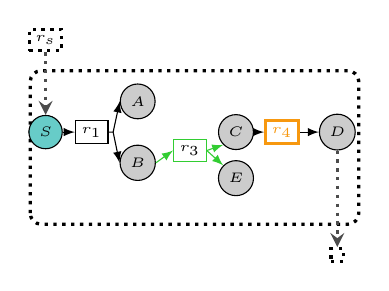
\begin{tikzpicture}[scale=0.39]\tiny
      \tikzstyle{metabolite}=[draw,circle,fill=white!80!black];
      \tikzstyle{repairmetabolite}=[draw,white!40!black, circle,fill=white!90!black,text=white!40!black,dashed];
      \tikzstyle{seed}=[draw,circle,fill=BlueGreen!70];%white!80!black
      \tikzstyle{target}=[draw,circle,fill=YellowOrange];%white!40!black
      \tikzstyle{reaction}=[draw,rectangle];
       \tikzstyle{export}=[draw,rectangle,dotted, very thick];
       \tikzstyle{exportrepair}=[draw,rectangle,dotted, very thick,white!80!black,text=white!70!black];
      \tikzstyle{repairreaction}=[draw,rectangle,white!40!black,text=white!40!black,dashed];
      \tikzstyle{solreaction}=[draw,rectangle,LimeGreen,text=black];
      \tikzstyle{initial}=[->,>=latex,thick];
      \tikzstyle{bdd}=[->,>=latex,thick];
      \tikzstyle{etiq}=[midway,fill=black!20,scale=0.5];
      \tikzstyle{stc}=[draw, rectangle, white, text=black]


      \draw [black,dotted, rounded corners, very thick] (-0.5,4) rectangle (10.2,9);
     % \node (system) [draw, rounded rectangle] at (0,0) {} (7cm,5cm);

      \node[seed] (S) at (0,7) {$S$};
      \node[metabolite] (A) at (3,8) {$A$};
      \node[metabolite] (B) at (3,6) {$B$};
      \node[metabolite] (C) at (6.2,7) {$C$};
      \node[metabolite] (D) at (9.5,7) {$D$};
      \node[metabolite] (E) at (6.2,5.5) {$E$};

      \node[reaction] (R1) at (1.5,7) {$r_{1}$};
      \node[reaction, very thick,YellowOrange] (R4) at (7.7,7) {$r_{4}$}; %LimeGreen
      %\node[solreaction] (R2) at (4.7,7.6) {$r_{2}$};
      \node[solreaction] (R3) at (4.7,6.4) {$r_{3}$};

      % R1 : S => A + B
      \draw[->,>=latex] (S.east) -- (R1.west);
      \draw[->,>=latex] (R1.east) -- (2.2,7) -- (A.west);
      \draw[->,>=latex] (2.2,7)  -- (B.west);

      % R2 : A => C
      %\draw[->,>=latex,LimeGreen] (A.east) -- (R2.west);
      %\draw[->,>=latex,LimeGreen] (R2.east) -- (C.north west);

      % R3 : B => C + E
      \draw[->,>=latex,LimeGreen] (B.east) -- (R3.west);
      \draw[->,>=latex,LimeGreen] (R3.east) -- (C.south west);
      \draw[->,>=latex,LimeGreen] (R3.east) -- (E.north west);

      % R4 : C => D
      \draw[->,>=latex] (C.east) -- (R4.west);
      \draw[->,>=latex] (R4.east) -- (D.west);

      %export G
      \node[export] (outD) at (9.5,3) {\ExportReaction};
      \draw[->,>=stealth,white!30!black,dotted, very thick] (D.south) --  (outD.north);

      %import S2
      \node[export] (inS) at (0,10) {$r_{s}$};
      \draw[->,>=stealth,white!30!black,dotted, very thick] (inS) --  (S.north);

  \end{tikzpicture}
% \end{figure}

% \end{document}

      \caption{Topological completion $R_1=\{r_3\}$ satisfies $r_4\in\Activity{t}{G_2}{\{S\}}$, but carries no flux, due to accumulation of compounds $A$ and $E$ that contradicts Eq.~\ref{eq:stoichiometric:equation}.\label{gra:union_nf_nf2}}
    \end{minipage}
    \begin{minipage}[t]{.32\textwidth}
      % \documentclass{article}
% \usepackage[dvipsnames]{xcolor}
% \usepackage{tikz}
% \usepackage{xcolor,colortbl}
% 
% \begin{document}
% 
% \newcommand{\gringo}{\textit{gringo}}
\newcommand{\clasp}{\textit{clasp}}
\newcommand{\clingo}{\textit{clingo}}
\newcommand{\asprin}{\textit{asprin}}
\newcommand{\asap}{\textit{teaspoon}}
\newcommand{\piclasp}{\textit{piclasp}}

\newcommand{\code}[1]{\lstinline[basicstyle=\ttfamily]{#1}}

\newcommand{\lw}[1]{\smash{\lower1.ex\hbox{#1}}}
\newcommand{\llw}[1]{\smash{\lower3.ex\hbox{#1}}}

%\newcommand{\dataCL}[5]{%
%  \code{#1} & #3 & #5 & #4
%}
%\newcommand{\dataCS}[5]{%
%  #3 & #5 & #4
%}

\newenvironment{tableC}{%
  \scriptsize
  \tabcolsep = 0.6mm
  \begin{tabular}[t]{l|rlr|rlr|rlr|rlr|rlr}\hline
    \multicolumn{1}{l|}{\llw{Instance}} &
    \multicolumn{3}{c|}{UD1} &
    \multicolumn{3}{c|}{UD2} &
    \multicolumn{3}{c|}{UD3} &
    \multicolumn{3}{c|}{UD4} &
    \multicolumn{3}{c}{UD5} \\
    & 
    \multicolumn{1}{c}{Best} & & \multicolumn{1}{c|}{\emph{tea-}} & 
    \multicolumn{1}{c}{Best} & & \multicolumn{1}{c|}{\emph{tea-}} & 
    \multicolumn{1}{c}{Best} & & \multicolumn{1}{c|}{\emph{tea-}} & 
    \multicolumn{1}{c}{Best} & & \multicolumn{1}{c|}{\emph{tea-}} & 
    \multicolumn{1}{c}{Best} & & \multicolumn{1}{c}{\emph{tea-}} \\
    & 
    known & & \emph{spoon} & 
    known & & \emph{spoon} & 
    known & & \emph{spoon} & 
    known & & \emph{spoon} & 
    known & & \emph{spoon} \\
    \hline
  }{%
    \hline
  \end{tabular}
}

\newenvironment{tableB}{%
  \scriptsize
  \tabcolsep = 0.7mm
%  \begin{tabular}[t]{|l|c|r|l|l|l|}\hline
  \begin{tabular}[t]{lcrlll}\hline
    Instance &
    Formulation &
    Time (sec.)\\
    \hline
  }{%
    \hline
  \end{tabular}
}
\newenvironment{tableL}{%
  \scriptsize
  \tabcolsep = 0.7mm
  \begin{tabular}[t]{l|rrrrrrrr|r}\hline
    \lw{Instance} &
    \lw{Time (sec.)} &
    \multicolumn{6}{c}{The best utility vector} &
    The sum of  &
    The best of basic\\
    &
    &
    $(S_1,$ & $S_4,$ & $S_2,$ & $S_7,$ & $S_6,$ & $S_3)$ &
    utility vector &
    and optimized \\
    \hline
  }{%
    \hline
  \end{tabular}
}

%%% Local Variables:
%%% mode: latex
%%% TeX-master: "paper"
%%% End:


% \begin{figure}[t]
%   \centering

    \usetikzlibrary{shapes.misc, positioning}
    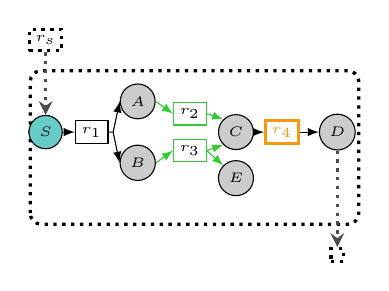
\begin{tikzpicture}[scale=0.39]\tiny
      \tikzstyle{metabolite}=[draw,circle,fill=white!80!black];
      \tikzstyle{repairmetabolite}=[draw,white!40!black, circle,fill=white!90!black,text=white!40!black,dashed];
      \tikzstyle{seed}=[draw,circle,fill=BlueGreen!70];%white!80!black
      \tikzstyle{target}=[draw,circle,fill=YellowOrange];%white!40!black
      \tikzstyle{reaction}=[draw,rectangle];
       \tikzstyle{export}=[draw,rectangle,dotted, very thick];
       \tikzstyle{exportrepair}=[draw,rectangle,dotted, very thick,white!80!black,text=white!70!black];
      \tikzstyle{repairreaction}=[draw,rectangle,white!40!black,text=white!40!black,dashed];
      \tikzstyle{solreaction}=[draw,rectangle,LimeGreen,text=black];
      \tikzstyle{initial}=[->,>=latex,thick];
      \tikzstyle{bdd}=[->,>=latex,thick];
      \tikzstyle{etiq}=[midway,fill=black!20,scale=0.5];
      \tikzstyle{stc}=[draw, rectangle, white, text=black]


      \draw [black,dotted, rounded corners, very thick] (-0.5,4) rectangle (10.2,9);
     % \node (system) [draw, rounded rectangle] at (0,0) {} (7cm,5cm);

      \node[seed] (S) at (0,7) {$S$};
      \node[metabolite] (A) at (3,8) {$A$};
      \node[metabolite] (B) at (3,6) {$B$};
      \node[metabolite] (C) at (6.2,7) {$C$};
      \node[metabolite] (D) at (9.5,7) {$D$};
      \node[metabolite] (E) at (6.2,5.5) {$E$};

      \node[reaction] (R1) at (1.5,7) {$r_{1}$};
      \node[reaction, very thick,YellowOrange] (R4) at (7.7,7) {$r_{4}$}; %LimeGreen
      \node[solreaction] (R2) at (4.7,7.6) {$r_{2}$};
      \node[solreaction] (R3) at (4.7,6.4) {$r_{3}$};

      % R1 : S => A + B
      \draw[->,>=latex] (S.east) -- (R1.west);
      \draw[->,>=latex] (R1.east) -- (2.2,7) -- (A.west);
      \draw[->,>=latex] (2.2,7)  -- (B.west);

      % R2 : A => C
      \draw[->,>=latex,LimeGreen] (A.east) -- (R2.west);
      \draw[->,>=latex,LimeGreen] (R2.east) -- (C.north west);

      % R3 : B => C + E
      \draw[->,>=latex,LimeGreen] (B.east) -- (R3.west);
      \draw[->,>=latex,LimeGreen] (R3.east) -- (C.south west);
      \draw[->,>=latex,LimeGreen] (R3.east) -- (E.north west);

      % R4 : C => D
      \draw[->,>=latex] (C.east) -- (R4.west);
      \draw[->,>=latex] (R4.east) -- (D.west);

      %export G
      \node[export] (outD) at (9.5,3) {\ExportReaction};
      \draw[->,>=stealth,white!30!black,dotted, very thick] (D.south) --  (outD.north);

      %import S2
      \node[export] (inS) at (0,10) {$r_{s}$};
      \draw[->,>=stealth,white!30!black,dotted, very thick] (inS) --  (S.north);

  \end{tikzpicture}
% \end{figure}

% \end{document}

      \caption{Completion with the union $R_1\cup R_2=\{r_2,r_3\}$. $G=G_1\cup G_2$ satisfies $r_4\in\Activity{t}{G}{\{S\}}$, but contradicts minimality and carries no flux $r_4\not \in\Activity{s}{G}{\{S\}}$, due to accumulation of compound $E$ that contradicts Eq.~\ref{eq:stoichiometric:equation}.\label{gra:union_nf_nf}}
    \end{minipage}
\end{figure}
% ----------------------------------------------------------------------



%%% Local Variables:
%%% mode: latex
%%% TeX-master: "paper"
%%% End:
